\begin{figure}[h!]
\centering
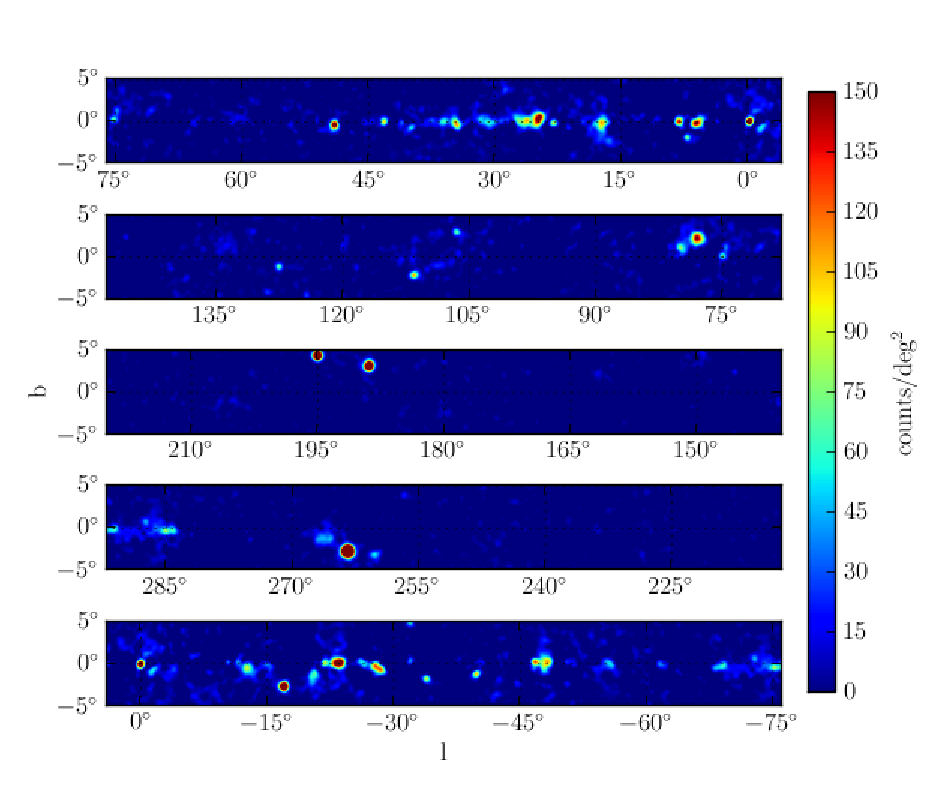
\includegraphics[width=\textwidth]{figures/Plan_gal.eps}
\caption{Residual counts map of the Galactic Plane above 10 GeV. The galactic and isotropic diffuse emission are subtracted using the files described in section 4.2 with a normalization of 1. All sources associated to Blazars are subtracted using the spectral parameters listed in the hard source list(+ citer Hard source list). Excesses visible in this map are due to Galactic sources emitting above 10 GeV observed by the LAT. The counts map is smoothed with a Gaussian of 0.27$\degr$.
\label{fig:PlanGal}}
\end{figure}

\begin{figure}[h!]
\centering
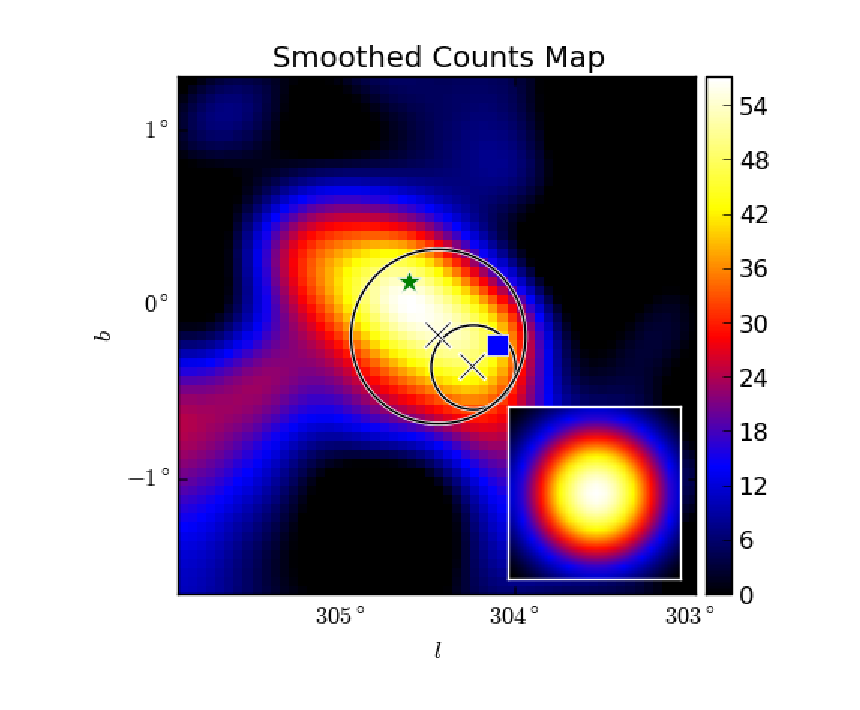
\includegraphics[]{figures/HESSJ1303m631.eps}
\caption{Counts map of the region of HESS~J1303--631. We subtracted the Galactic and isotropic diffuse emission. The counts map is smoothed by a 0.27$\degr$ gaussian corresponding to the PSF above 10 GeV. The green star show the position of the SNR Kes 17, the blue square represent the position of PSR~J1301--6305. The small and big circles respectively show the extension of TeV gaussian proposed by \cite{2005AA...439.1013A} and the extension of the disk derived in this work.
\label{1303}}
\end{figure}

\begin{figure}[h!]
\centering
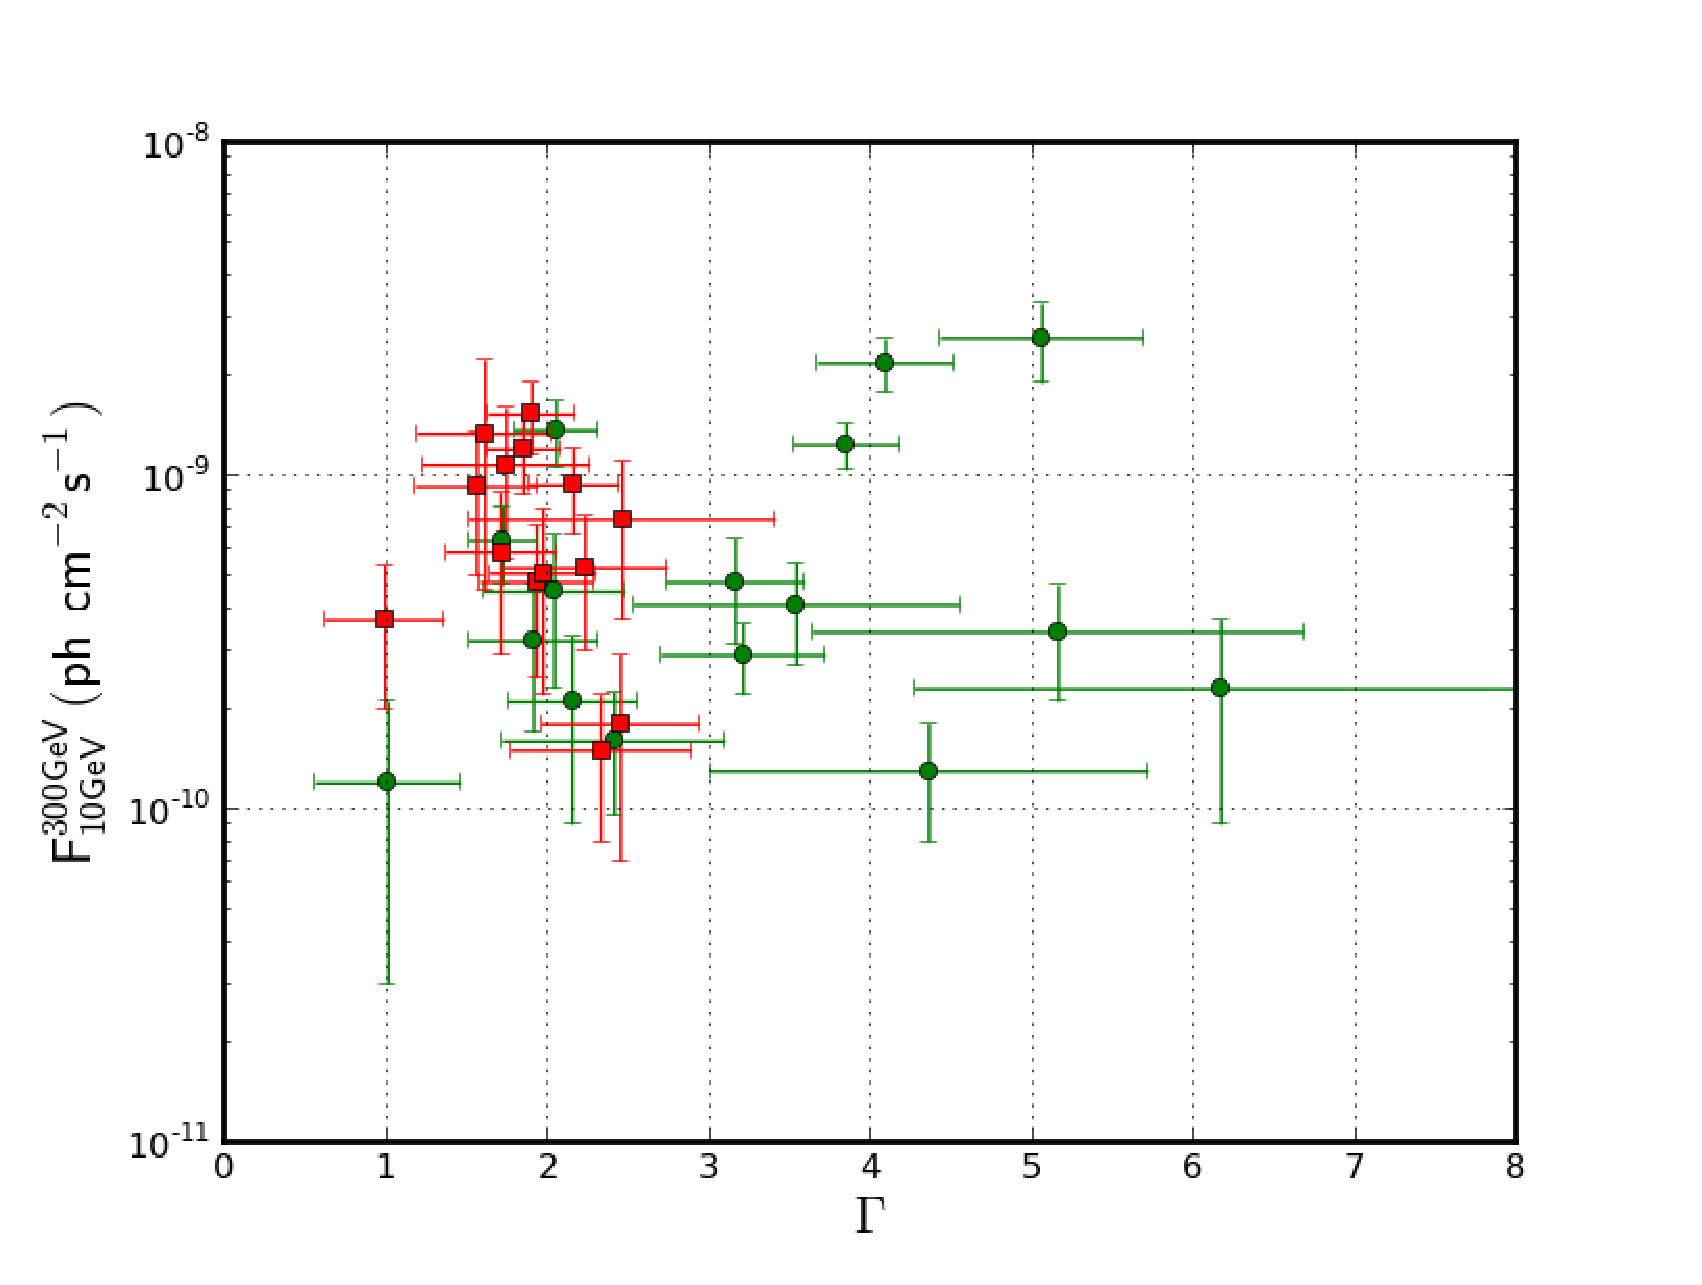
\includegraphics[width=\textwidth]{figures/out_errorbar_best_fit.eps}
\caption{Integrated flux of the detected sources as a function of the power-law index between 10 and 316 GeV. The green circles show the sources associated to pulsar detected by the LAT while the red squares represents the sources without pulsar detected in GeV energy ranges. The error bar shows the statistical and systematic uncertainties added in quadrature.  
\label{fig:fluxvssize}}
\end{figure}

\begin{figure}[h!]
\centering
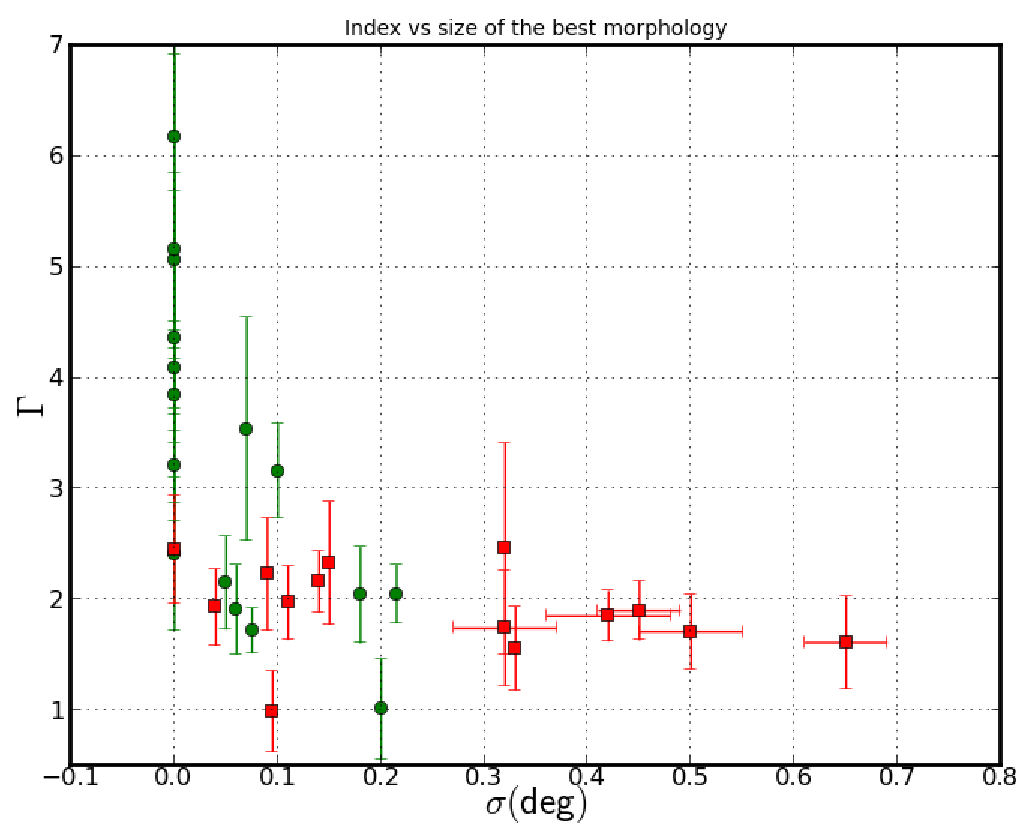
\includegraphics[width=\textwidth]{figures/index_vs_size.eps}
\caption{Index of the sources as a function of the extension found for each detected source. The green circles show the sources associated to pulsar detected by the LAT while the red squares represents the sources without pulsar detected in GeV energy ranges. The error bar shows the statistical and systematic uncertainties added in quadrature. 
\label{fig:indexvssize}}
\end{figure}

%\begin{figure}[h!]
%\centering
%\includegraphics[width=0.5\textwidth]{figures/0FGLJ1958.12848.eps}
%\caption{SED of MGRO J1958$+$2848. The red and blue points show respectively the \emph{Fermi}-LAT and ... points. The black error bars show the statistical and   systematic uncertainties added in quadrature. The black line corresponds to the best fit obtained using the LAT data. The dashed line correspond to the model of PSR J... taken from \cite{2012ApJS..199...31N}.
%\label{fig:1}}
%\end{figure}


\begin{figure}[h!]
\centering
\subfigure{
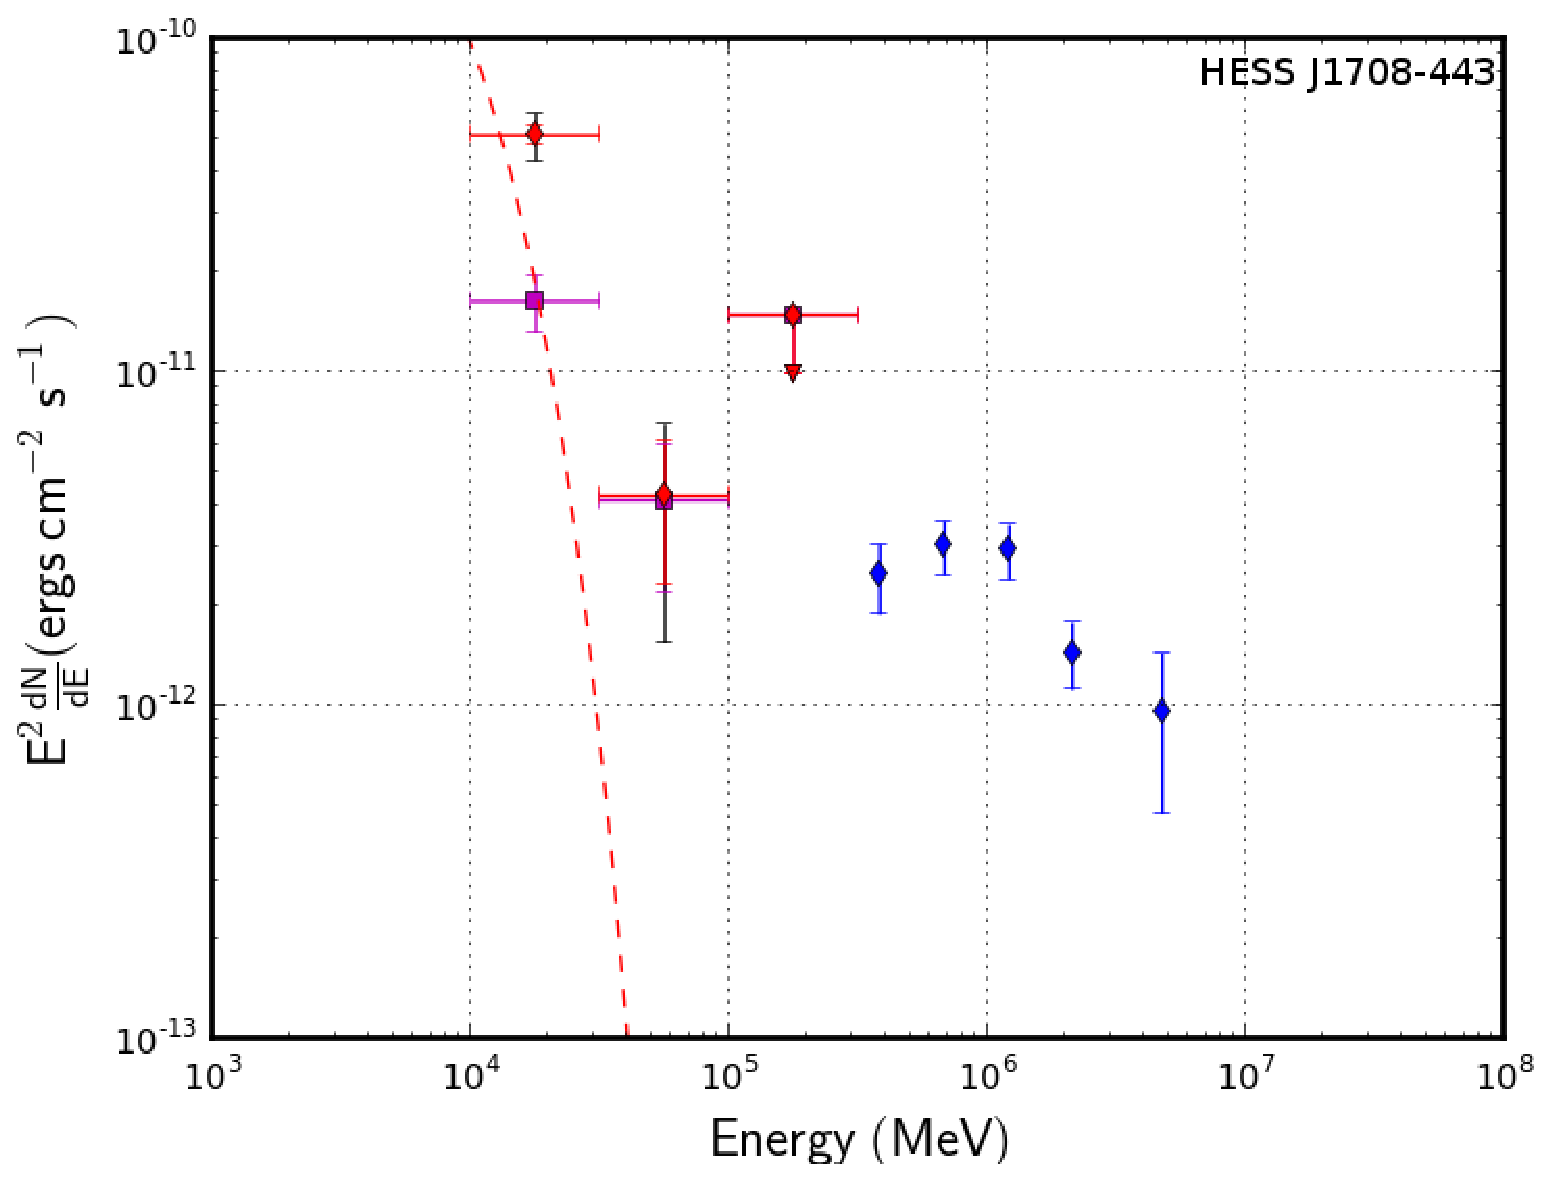
\includegraphics[width=0.45\textwidth]{figures/HESSJ1708.eps}
\label{fig:hess1708}
}
\subfigure{
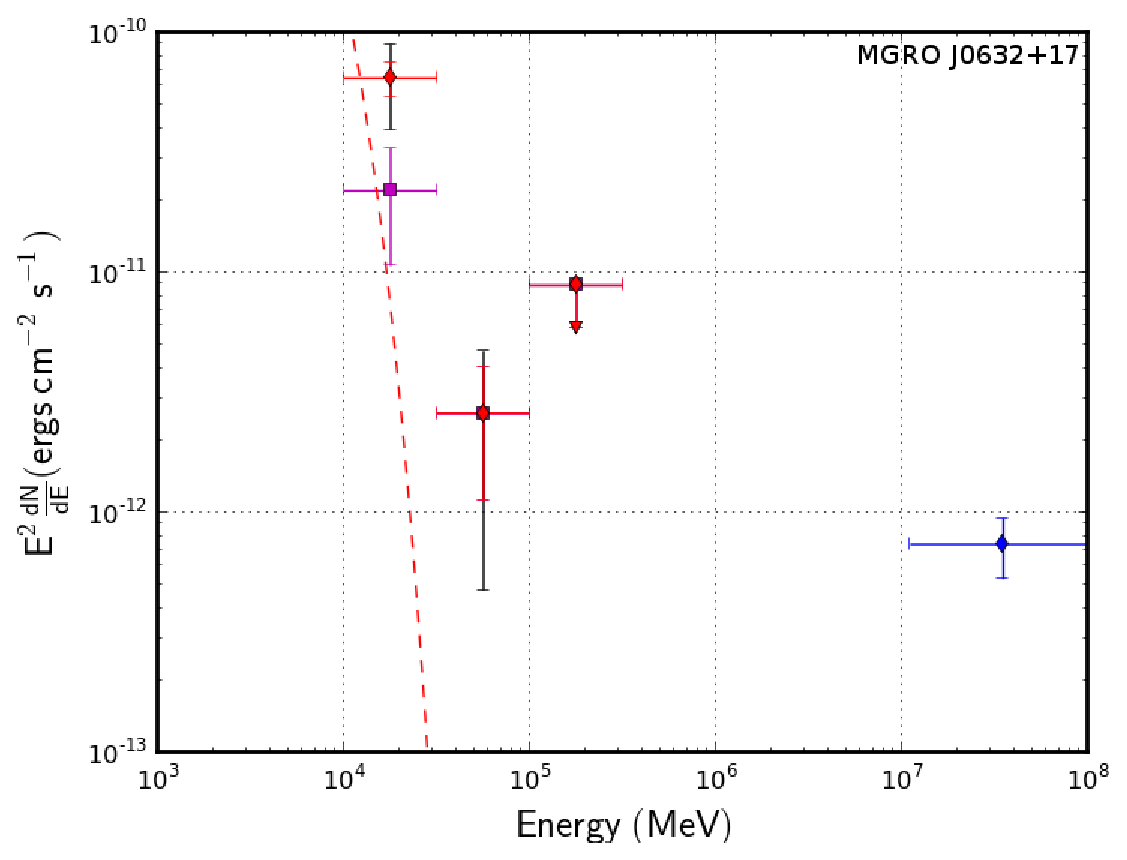
\includegraphics[width=0.45\textwidth]{figures/MGROJ0632.eps}
\label{fig:mgroj0632}
}
\subfigure{
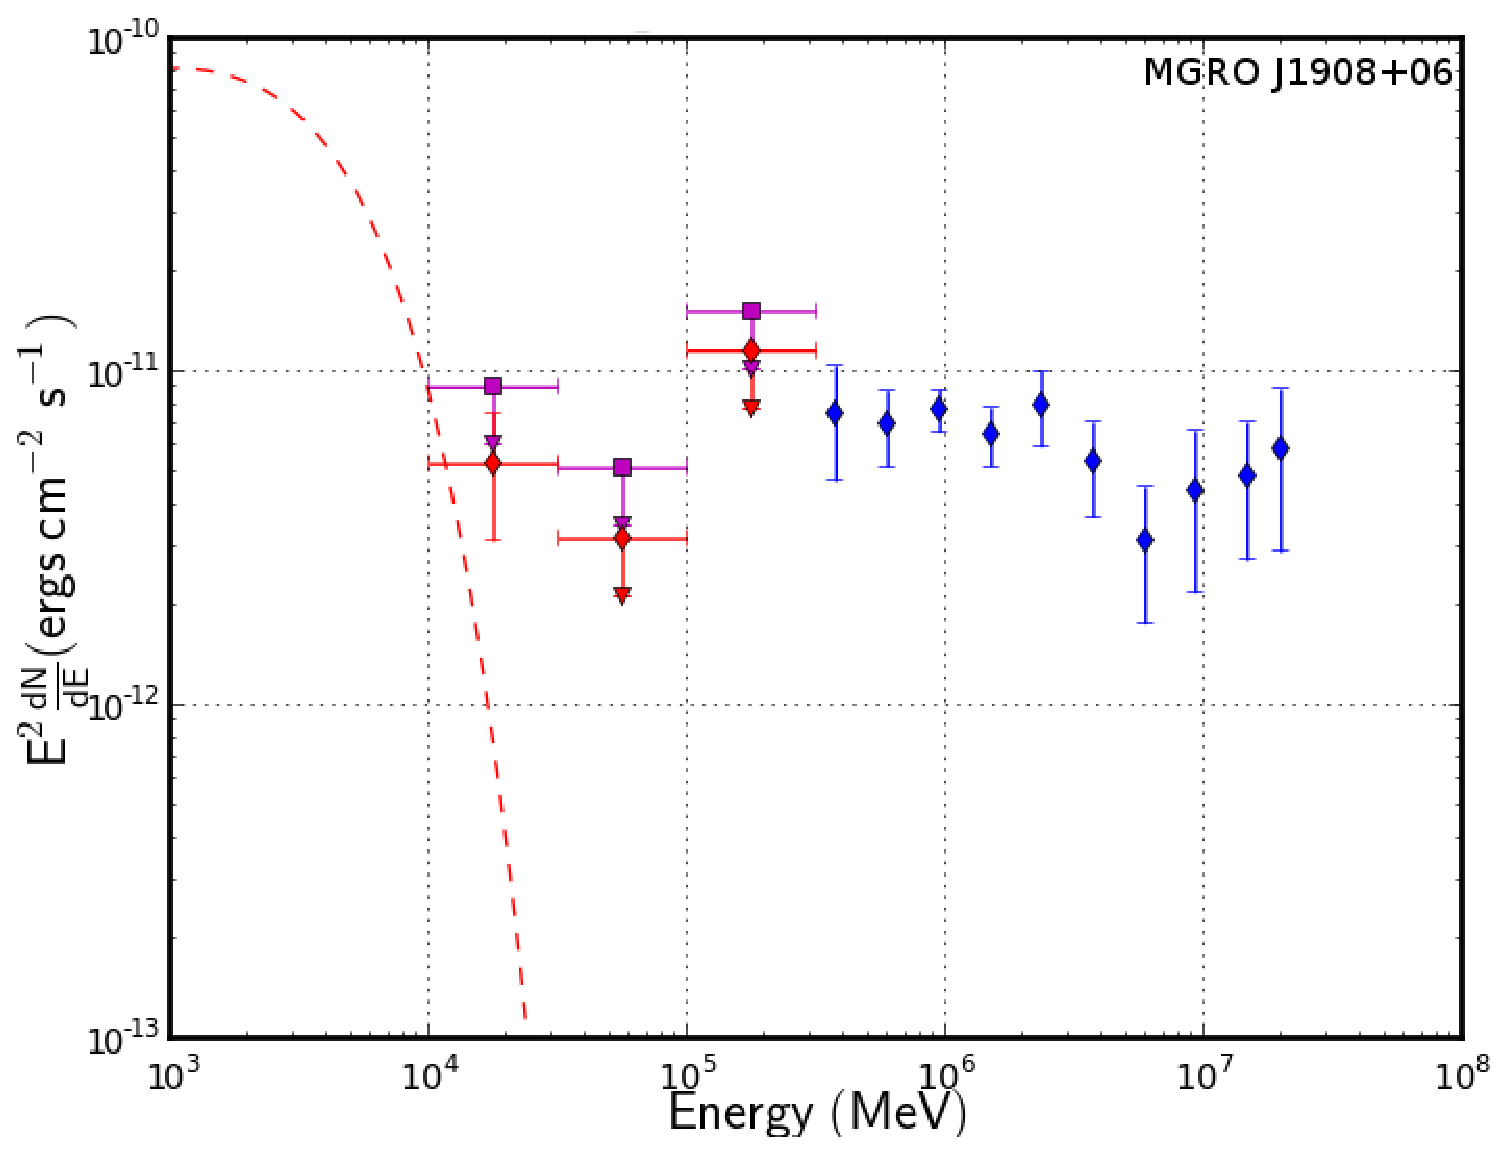
\includegraphics[width=0.45\textwidth]{figures/MGROJ1908.eps}
\label{fig:mgro1908}
}
\subfigure{
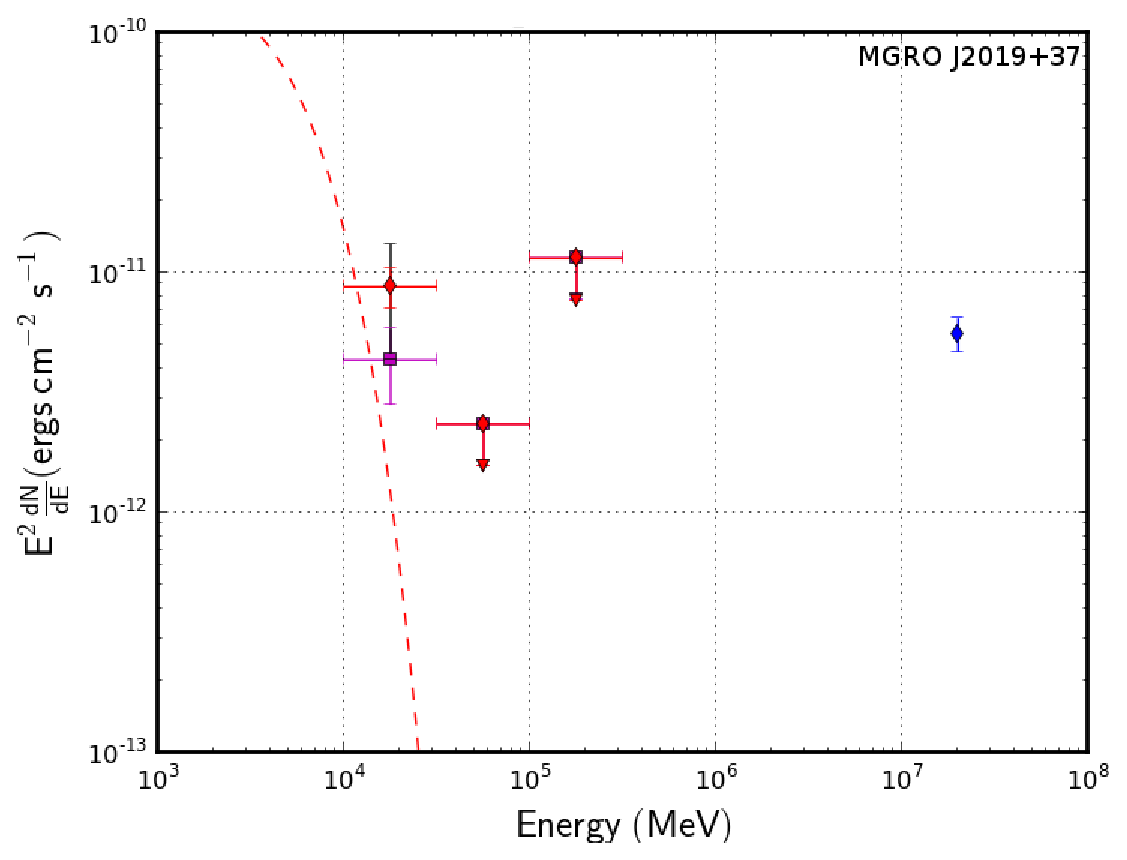
\includegraphics[width=0.45\textwidth]{figures/MGROJ201937.eps}
\label{fig:mgro2019}
}
\subfigure{
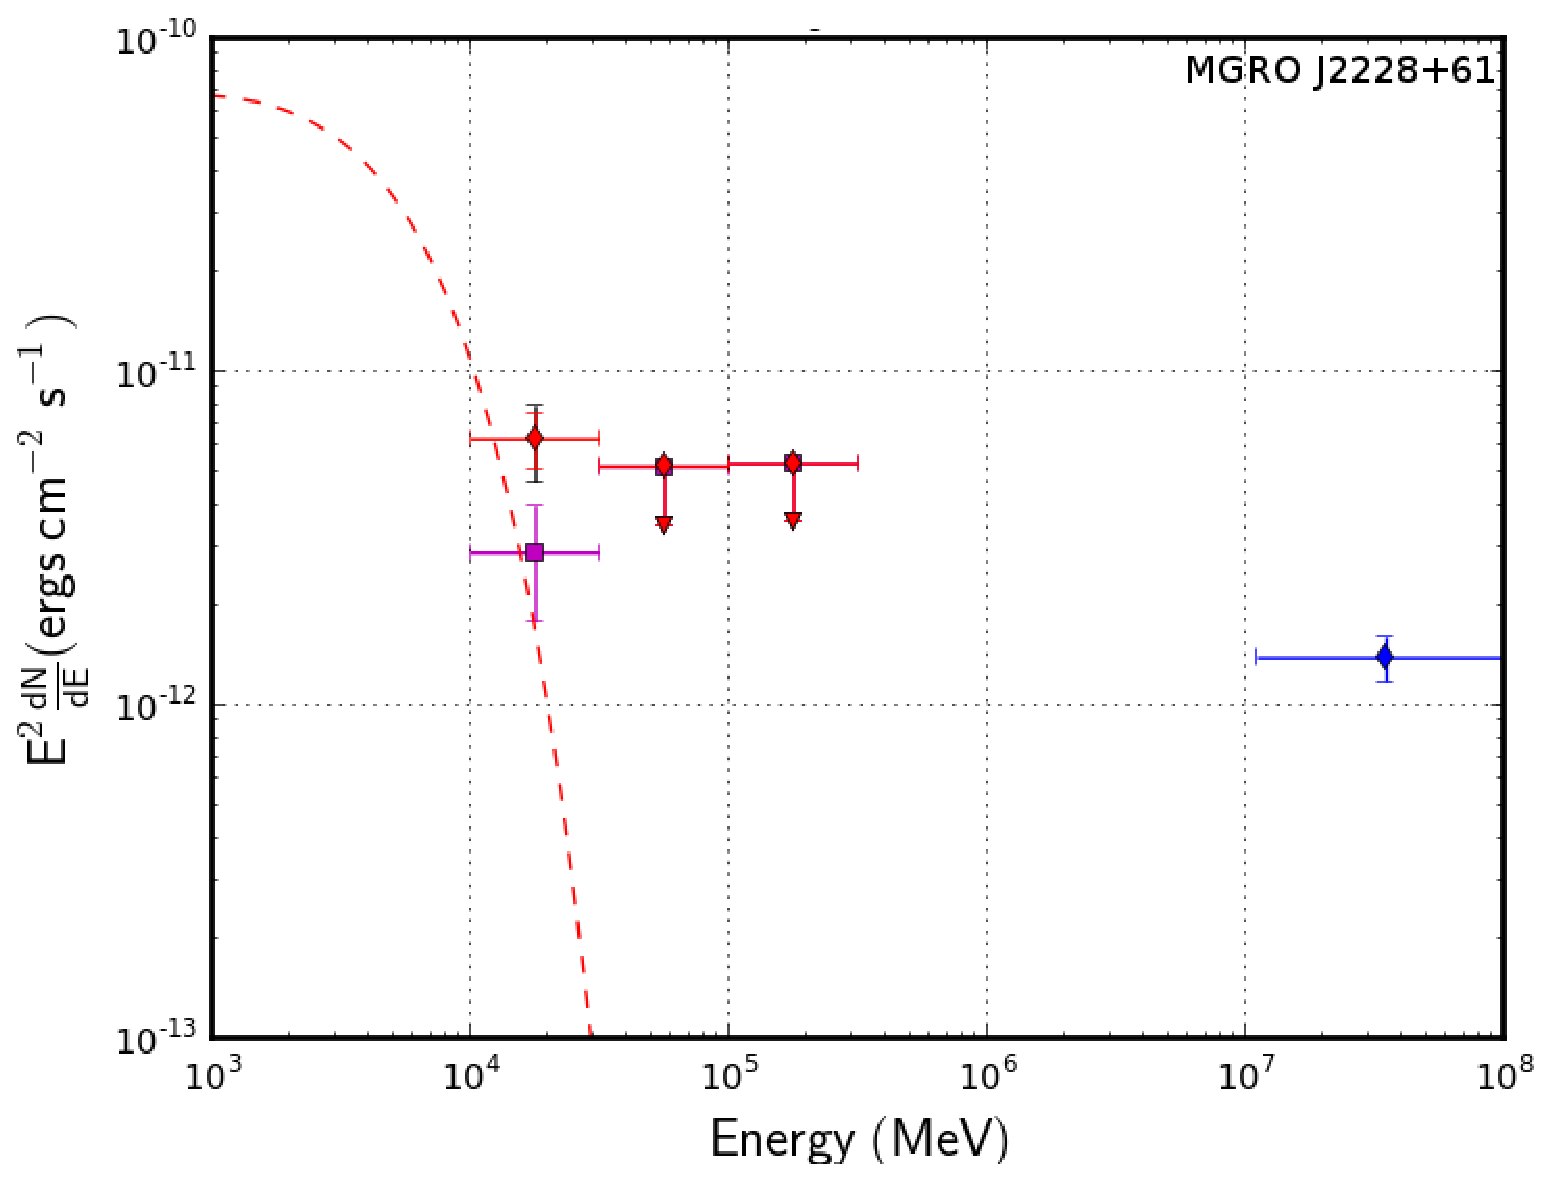
\includegraphics[width=0.45\textwidth]{figures/MGROJ2228.eps}
\label{fig:mgroj2228}
}
\subfigure{
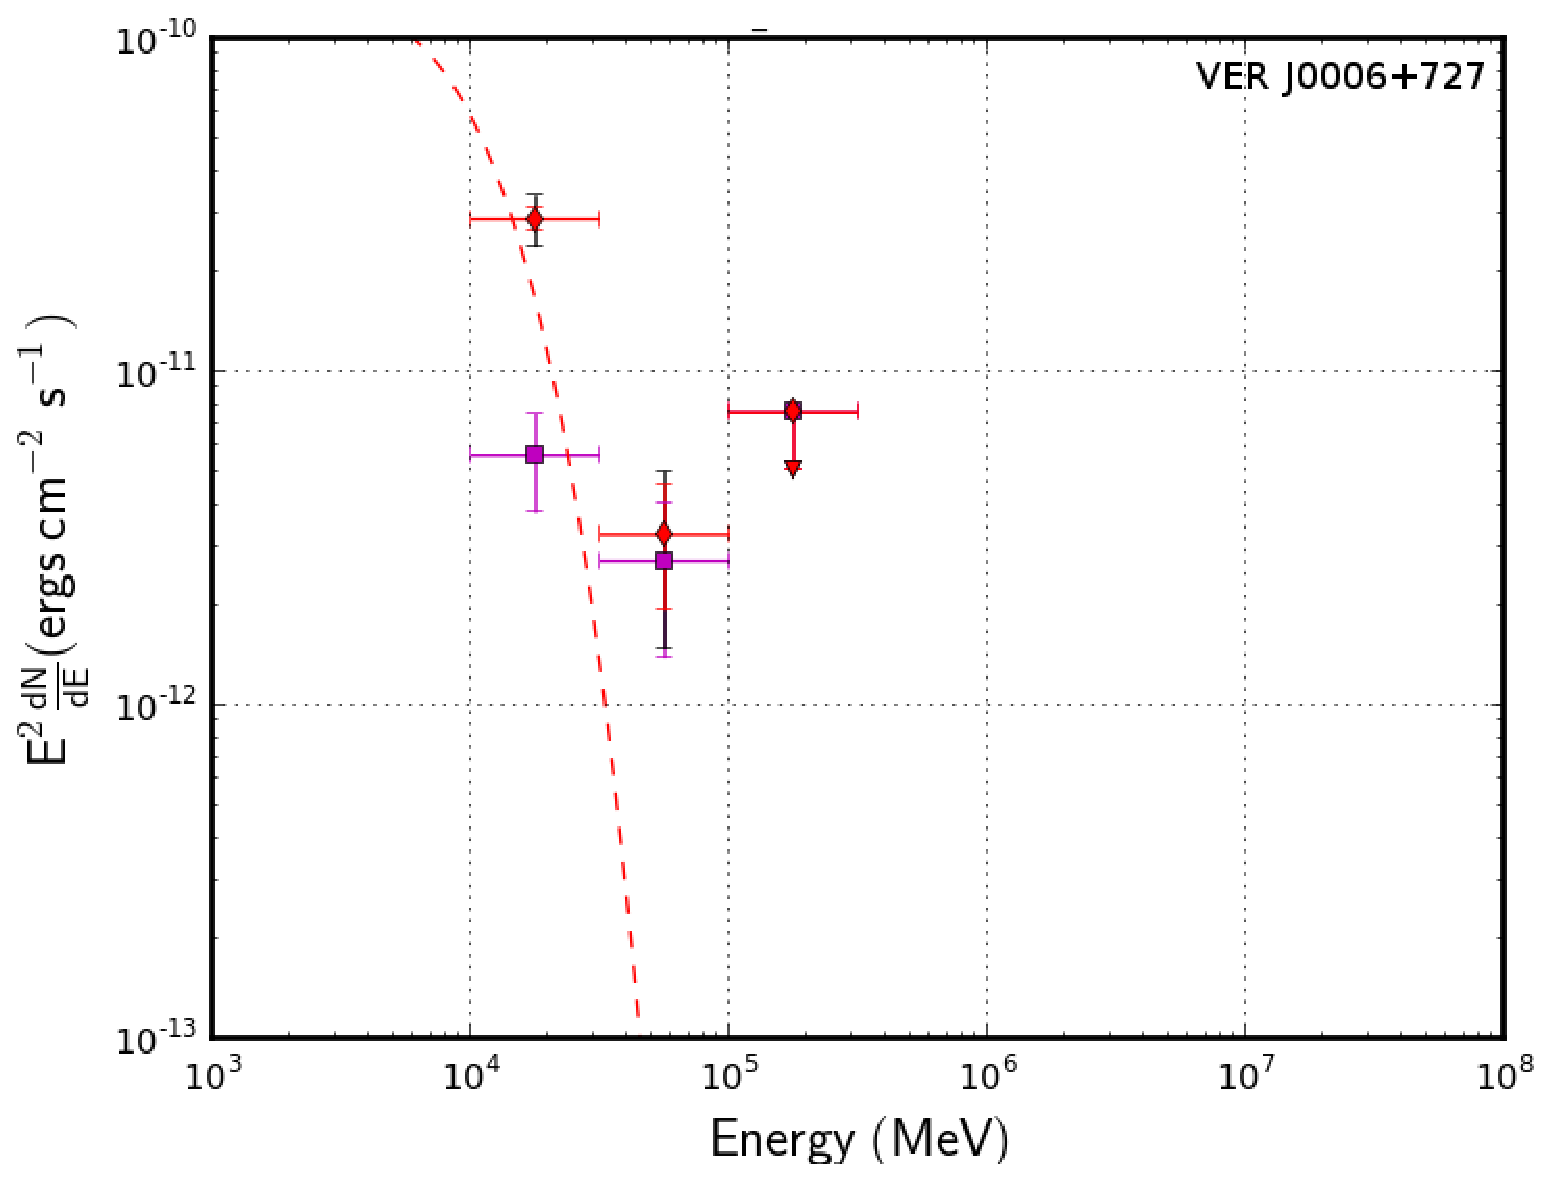
\includegraphics[width=0.45\textwidth]{figures/VERJ0006.eps}
\label{fig:verj0006}
}
\caption{\label{fig:sedsourcespuls}SED of the sources better described by a point--like source and with a pulsar within 0.5$\degr$. The blue points show the TeV points taken from \textbf{Add the papers}. The red circles and the magenta squares show respectively the SED without the pulsar included in the model and with the pulsar included in the model. The black error bars show the statistical and   systematic uncertainties added in quadrature. The dashed line correspond to the model of the associated pulsars sumarized in \ref{tab:pulsarfit} taken from \cite{2012ApJS..199...31N}. In the case of MGRO J1908+06, the red SED was derived assuming a point-like source as determined in tab. \ref{tab:GeVmorph} while the magenta SED was derived assuming the TeV shape.}
\end{figure}

\begin{figure}[h!]
\centering
\subfigure{
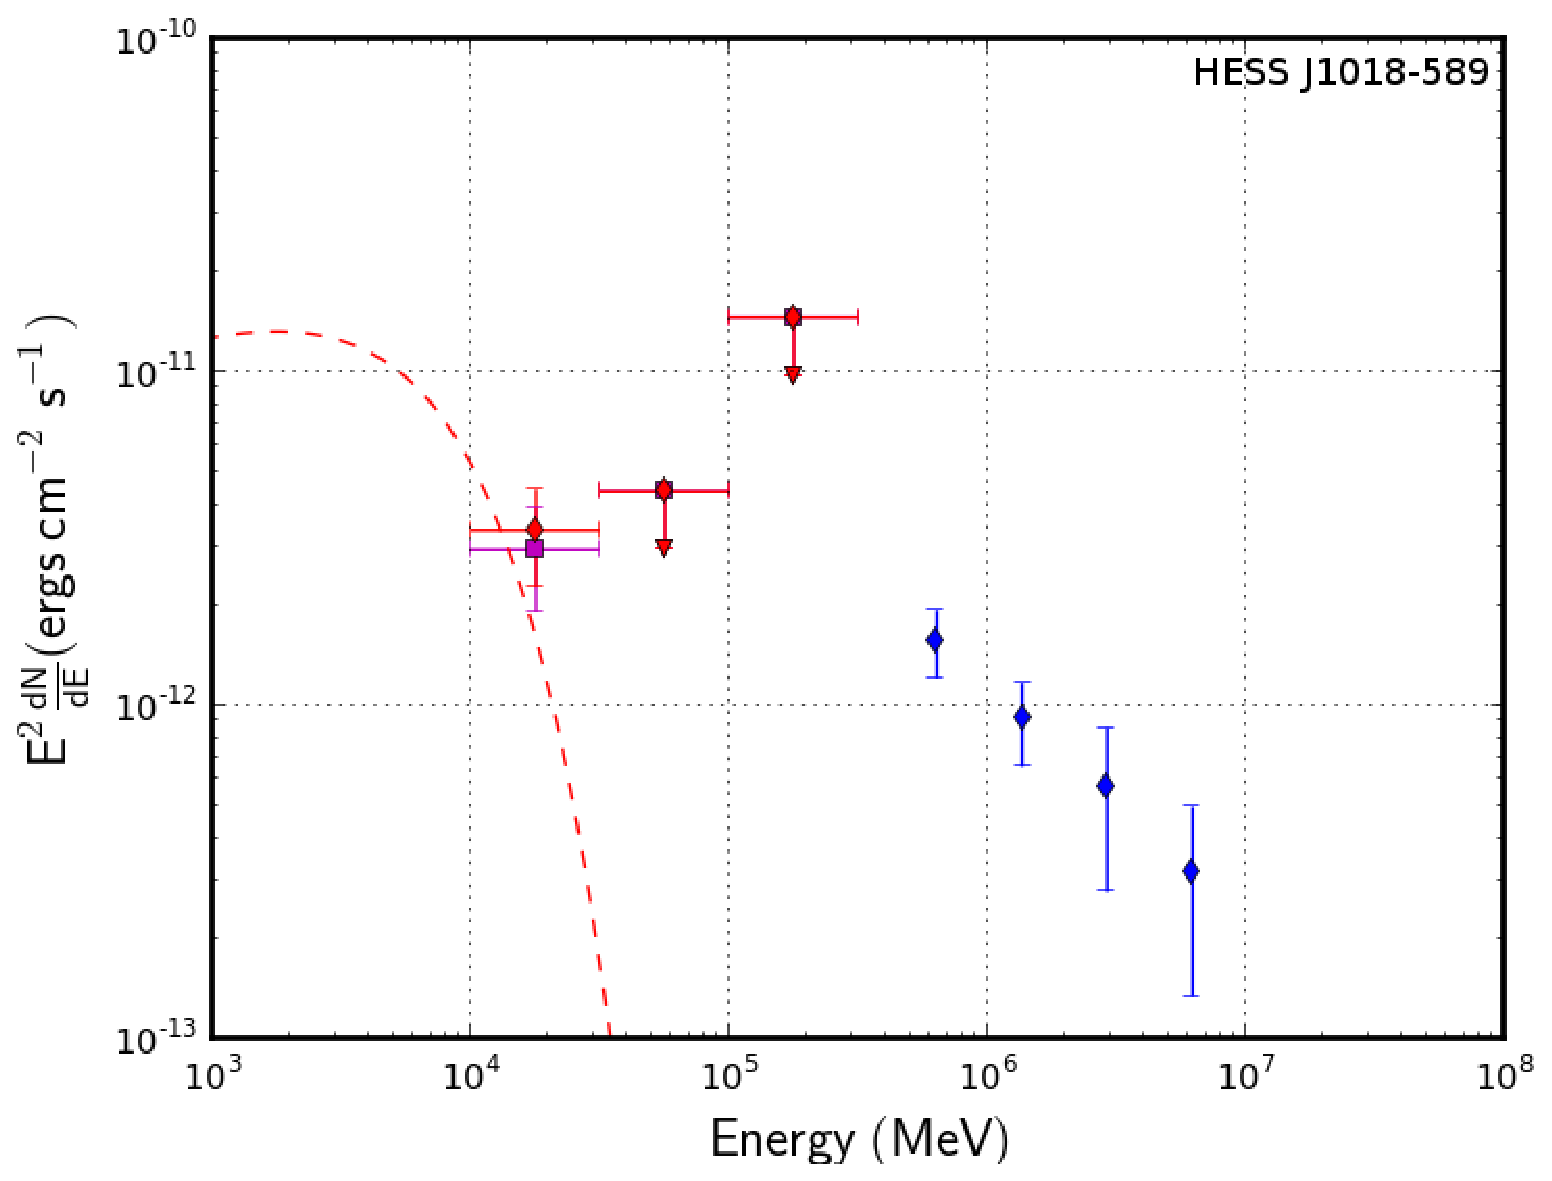
\includegraphics[width=0.45\textwidth]{figures/HESSJ1018.eps}
\label{fig:hessj1018}
}
\subfigure{
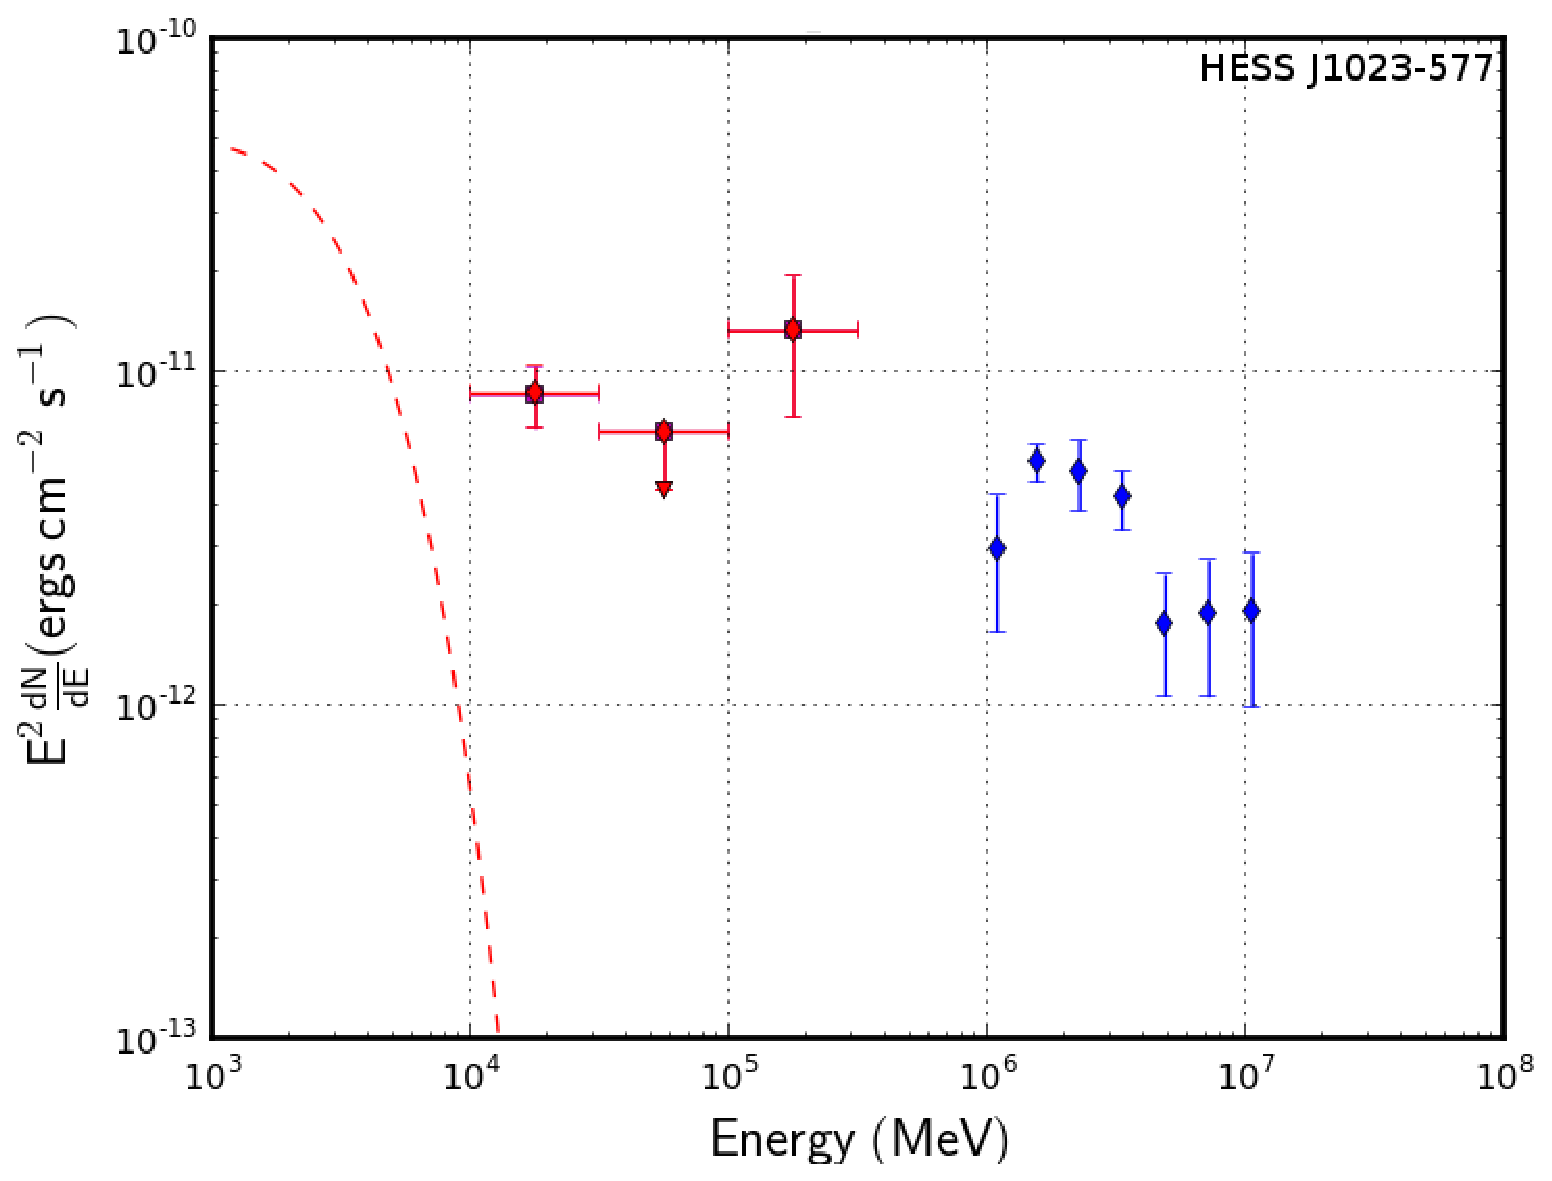
\includegraphics[width=0.45\textwidth]{figures/HESSJ1023.eps}
\label{fig:hessj1023}
}
\subfigure{
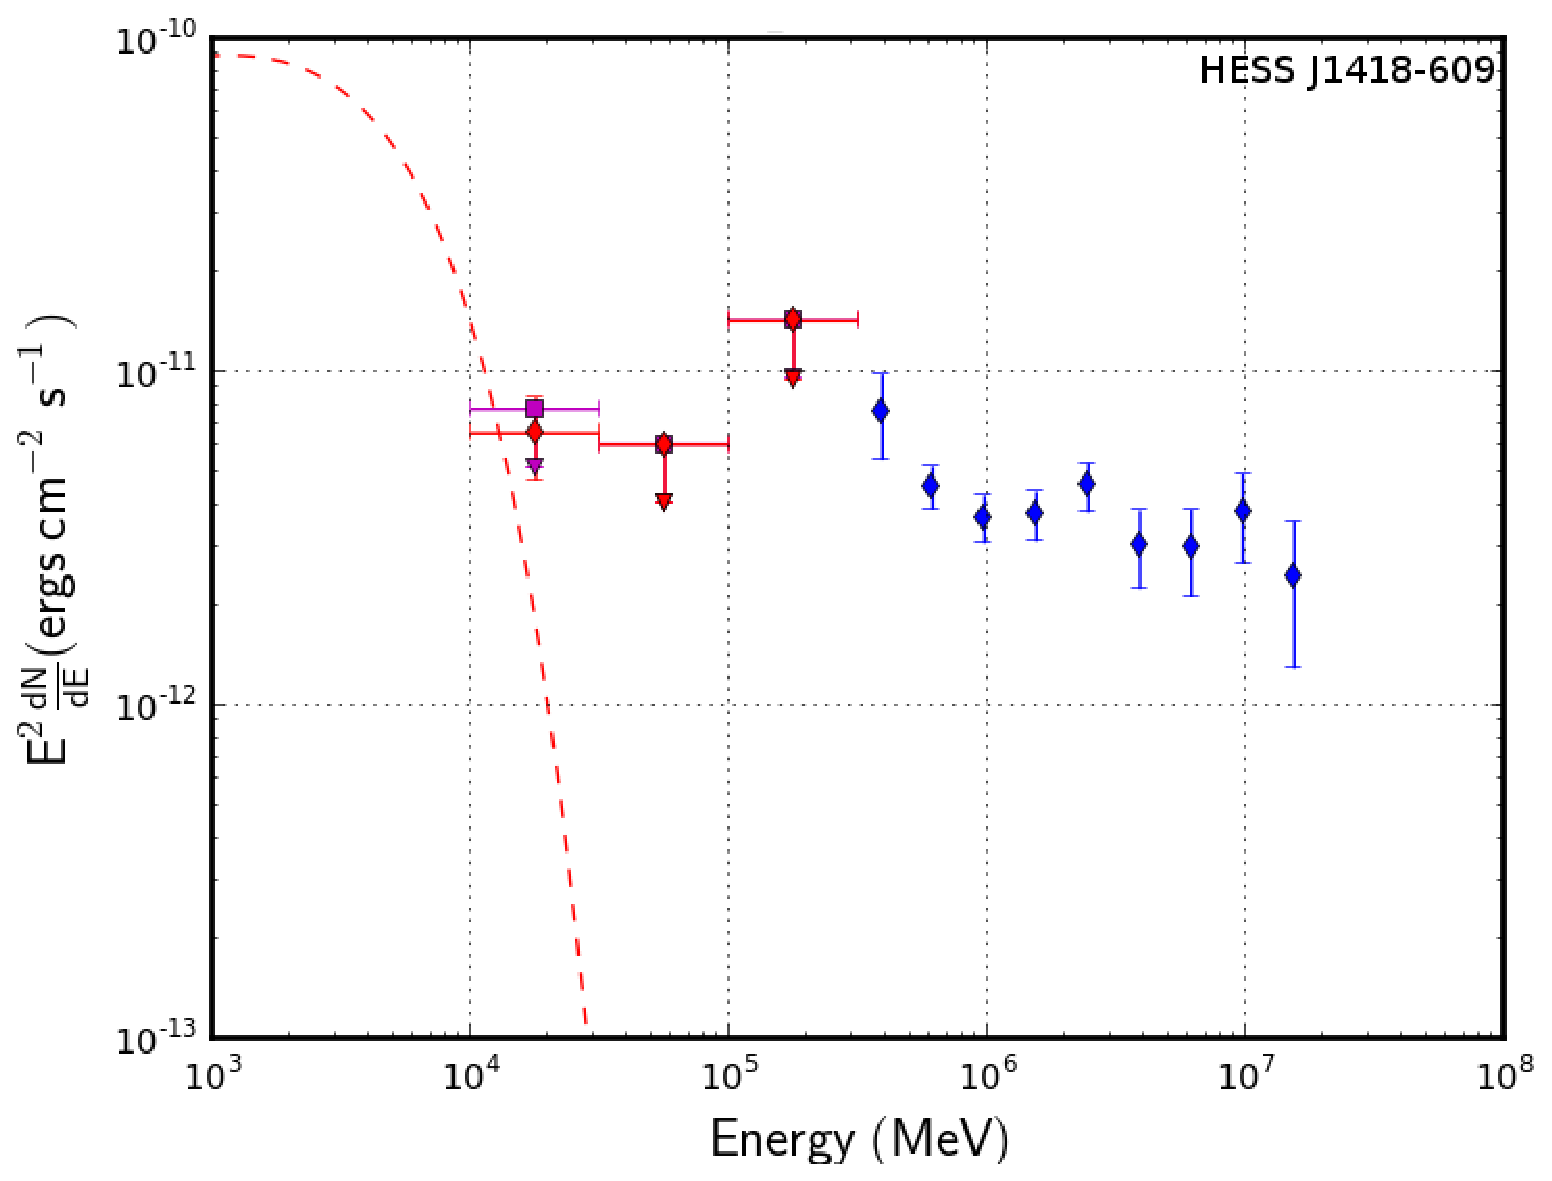
\includegraphics[width=0.45\textwidth]{figures/HESSJ1418.eps}
\label{fig:hessj1418}
}
\subfigure{
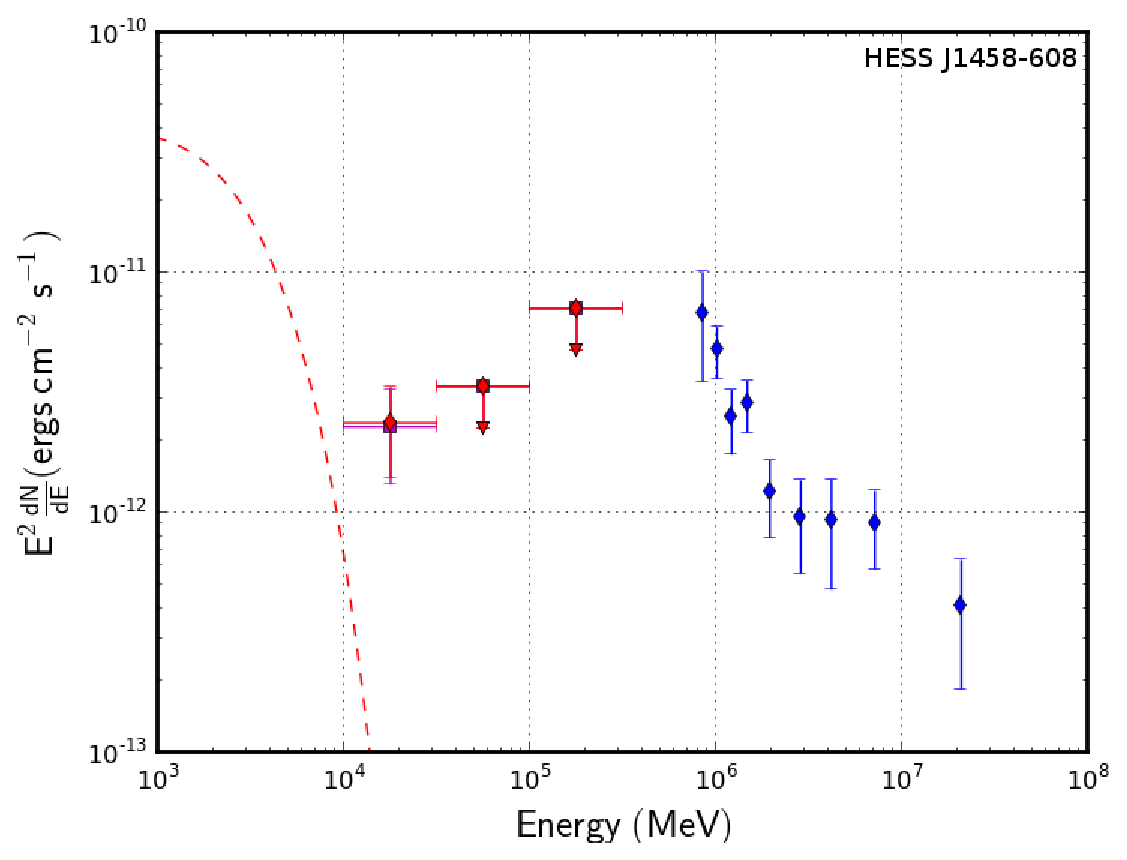
\includegraphics[width=0.45\textwidth]{figures/HESSJ1458.eps}
\label{fig:hessj1458}
}
\subfigure{
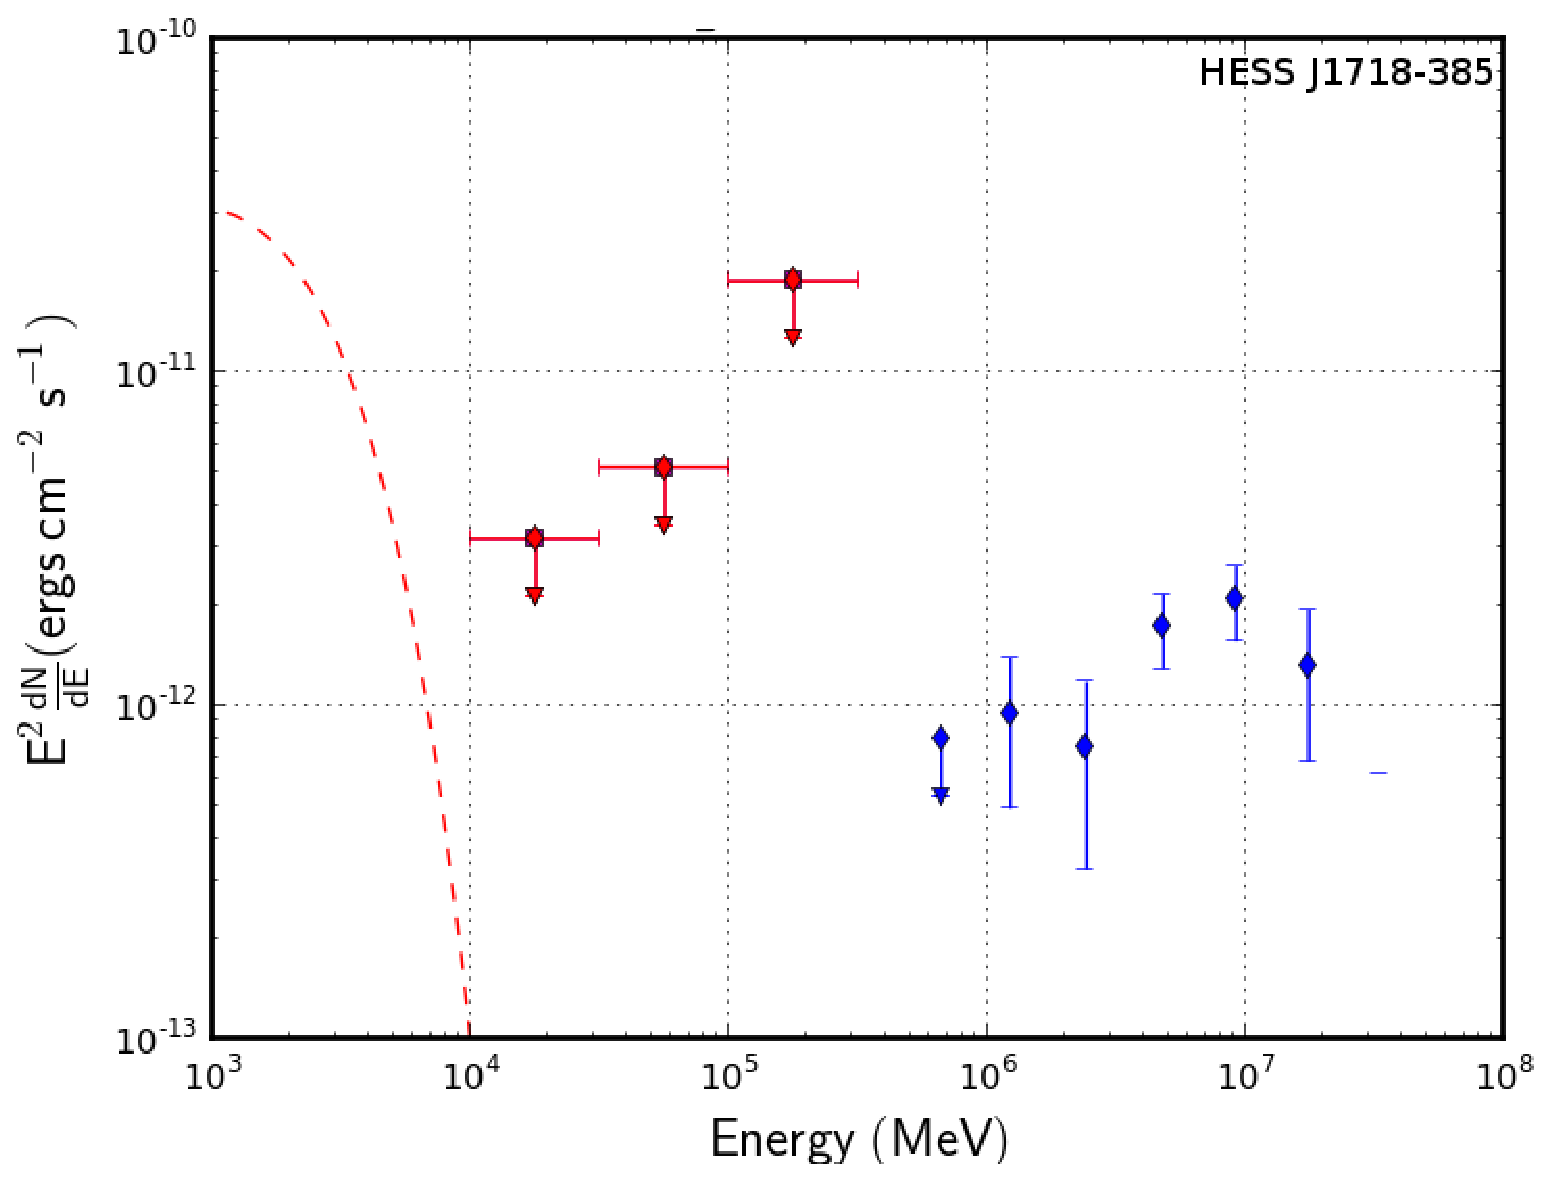
\includegraphics[width=0.45\textwidth]{figures/HESSJ1718.eps}
\label{fig:hessj1718}
}
\caption{\label{fig:sedsourcespuls2}SED of the sources better described by the TeV shape and with a pulsar within 0.5$\degr$. The blue points show the TeV points taken from \textbf{rajouter tous les papiers}. The red circles and the magenta squares show respectively the SED without the pulsar included in the model and with the pulsar included in the model. The black error bars show the statistical and   systematic uncertainties added in quadrature. The dashed line correspond to the model of the associated pulsars sumarized in \ref{tab:pulsarfit} taken from \cite{2012ApJS..199...31N}.}
\end{figure}

\begin{figure}[h!]
\centering

\subfigure{
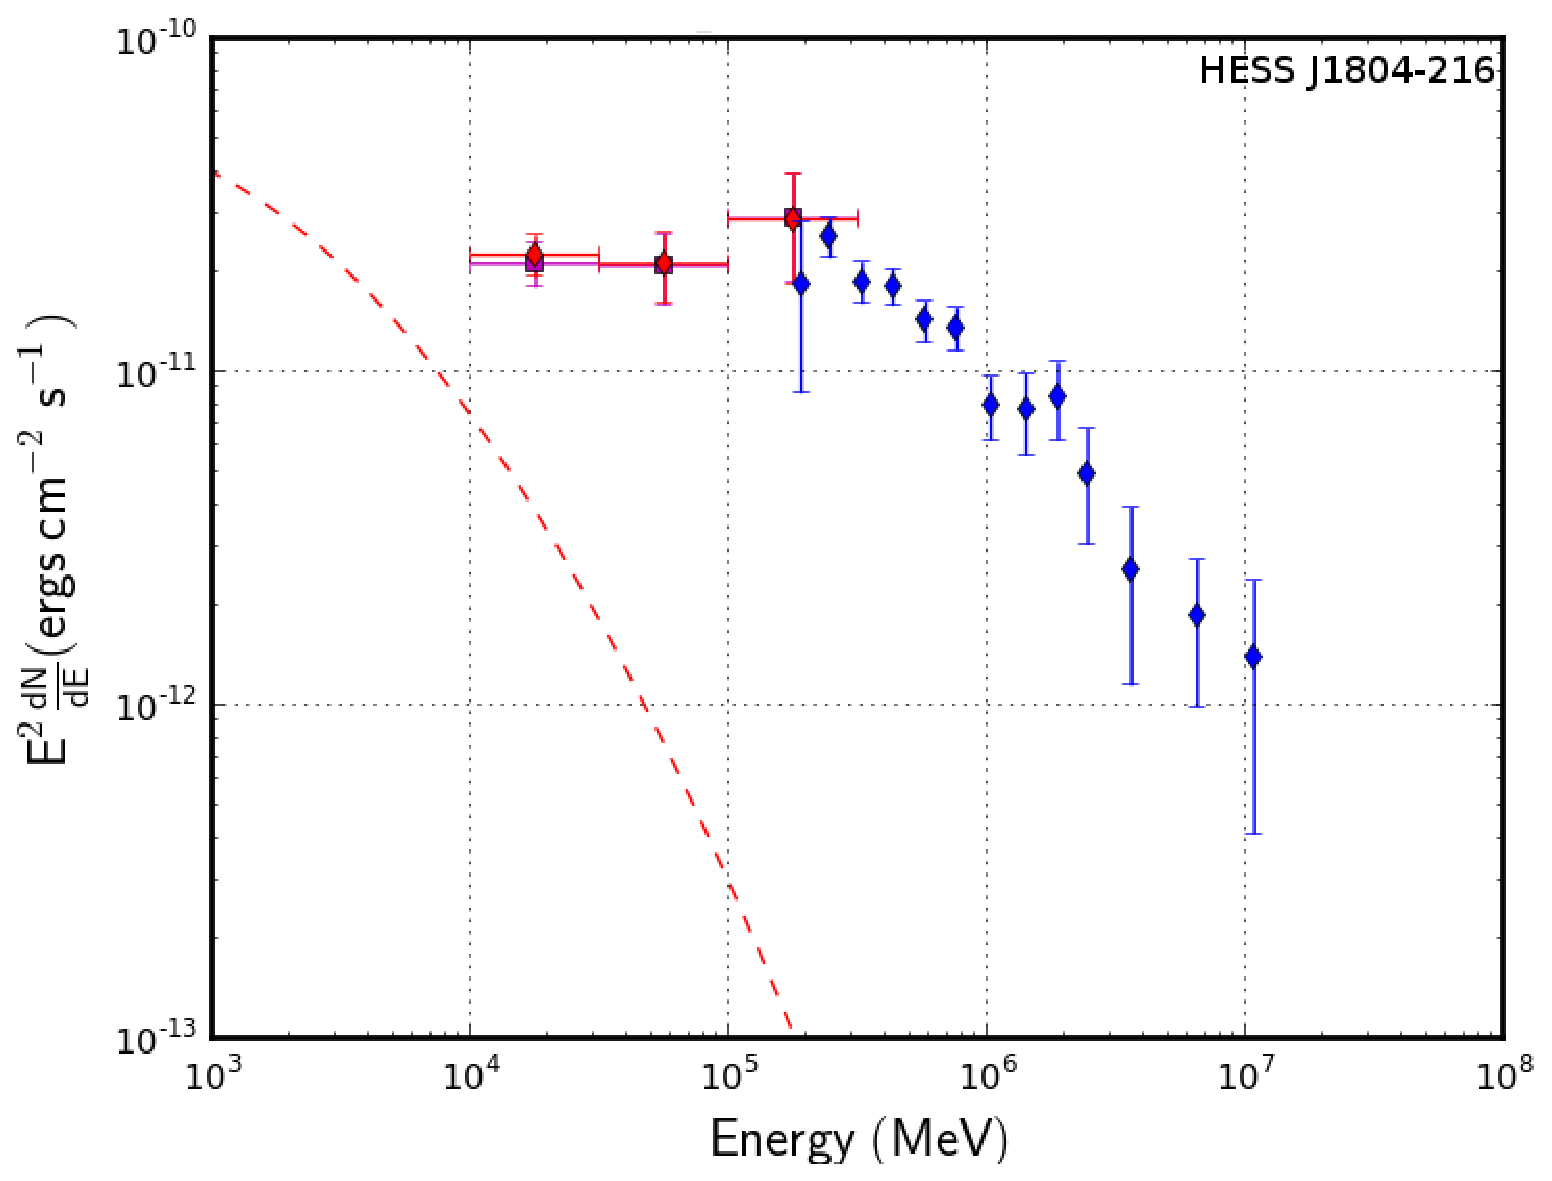
\includegraphics[width=0.45\textwidth]{figures/HESSJ1804.eps}
\label{fig:hessj1804}
}
\subfigure{
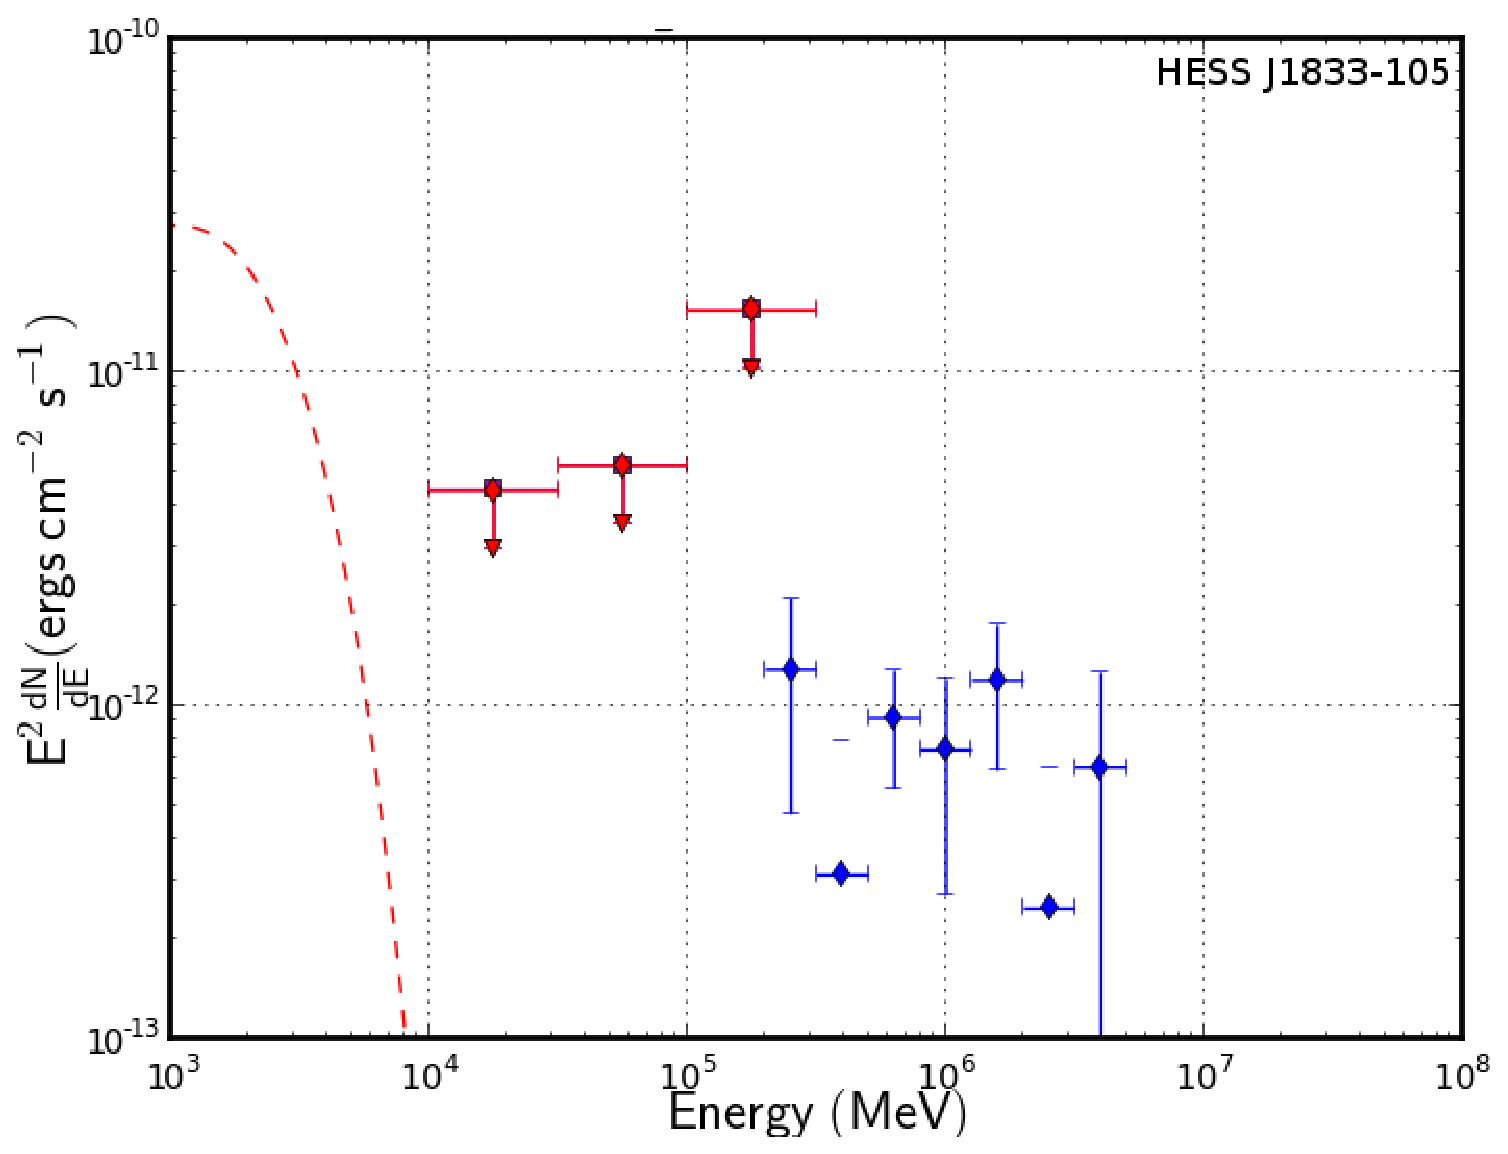
\includegraphics[width=0.45\textwidth]{figures/HESSJ1833.eps}
\label{fig:hess1833}
}
\subfigure{
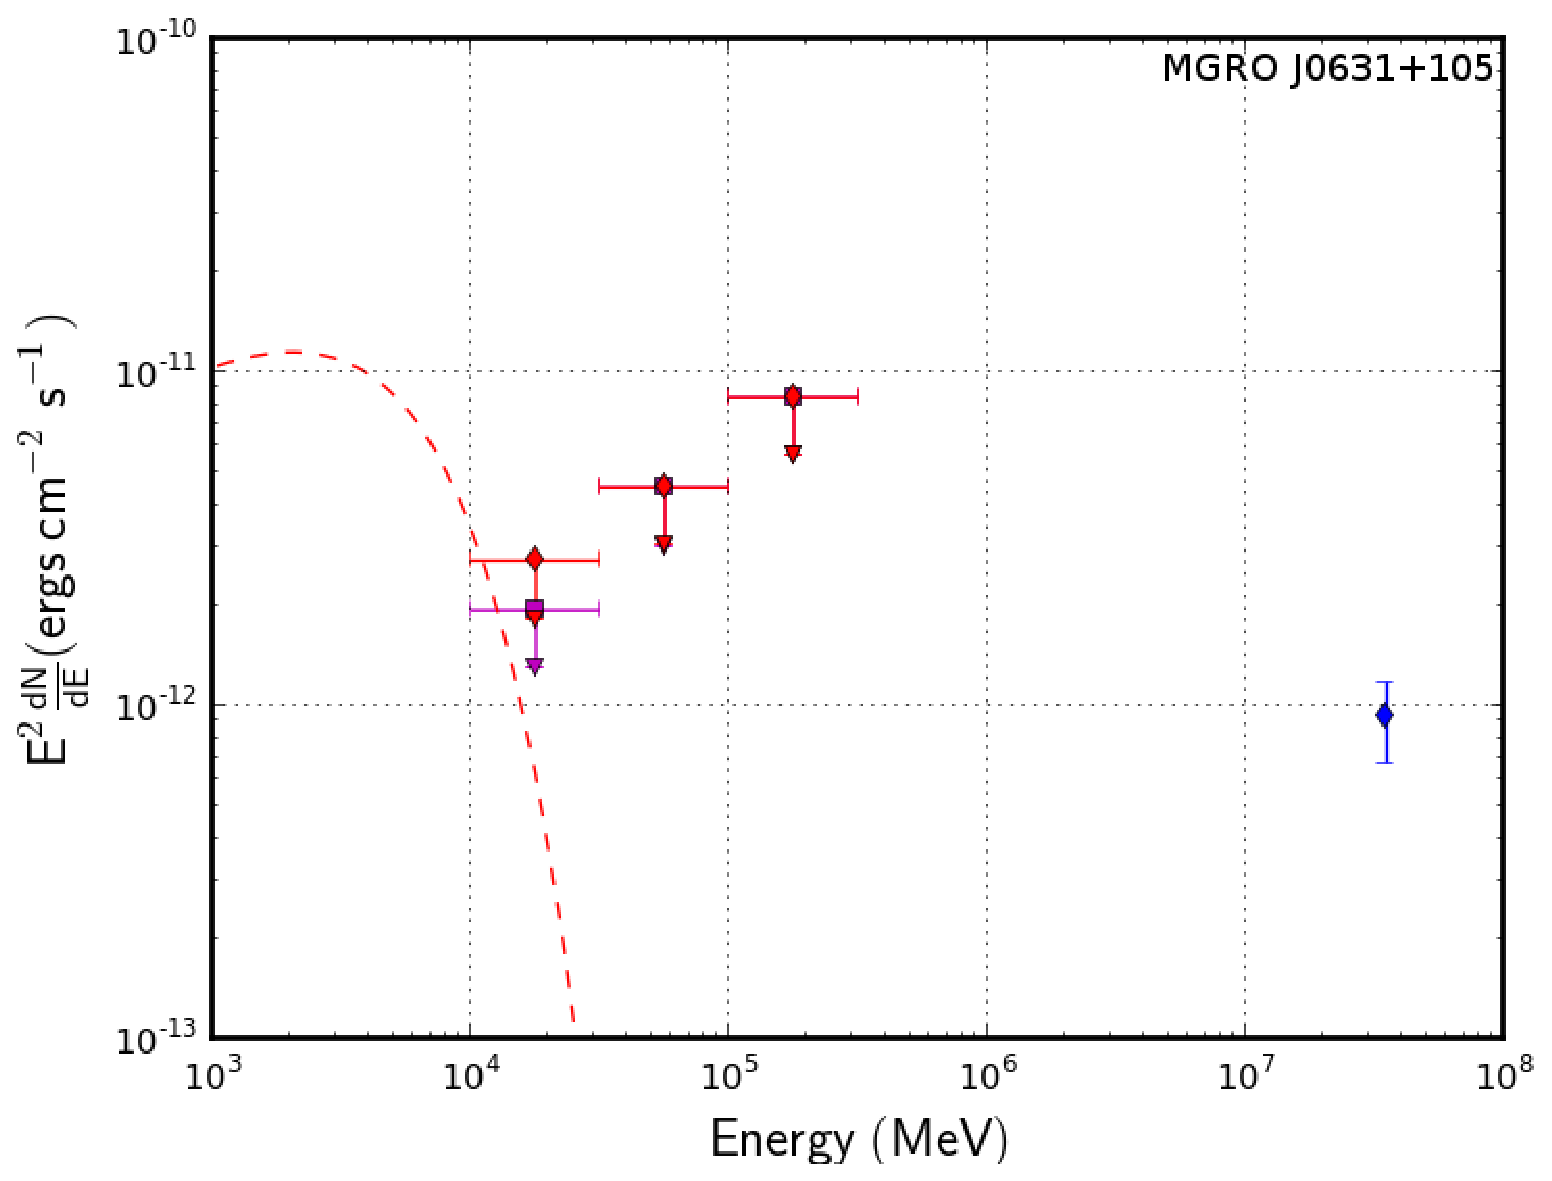
\includegraphics[width=0.45\textwidth]{figures/MGROJ0631.eps}
\label{fig:mgroj0631}
}
\subfigure{
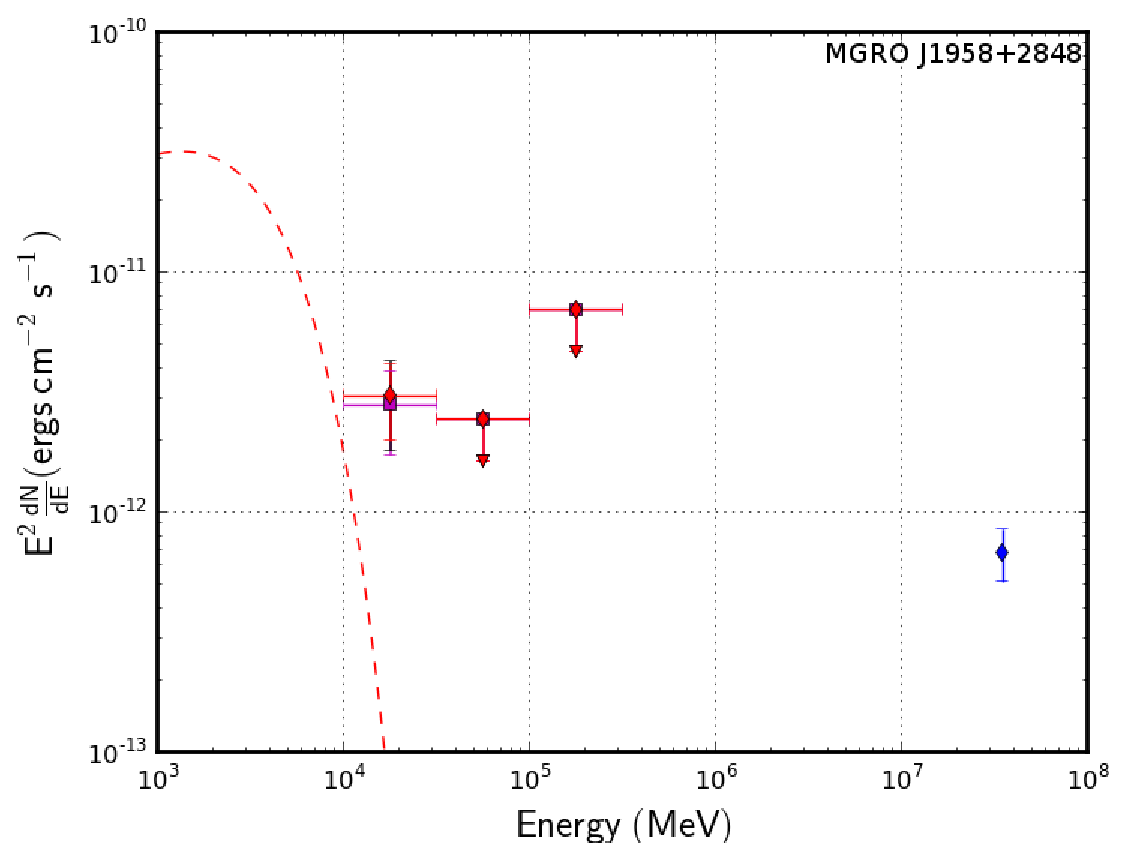
\includegraphics[width=0.45\textwidth]{figures/MGROJ1958.eps}
\label{fig:mgroj1958}
}

\caption{\label{fig:sedsourcespuls3}SED of the sources better described by the TeV shape and with a pulsar within 0.5$\degr$. The blue points show the TeV points taken from \textbf{rajouter tous les papiers}. The red circles and the magenta squares show respectively the SED without the pulsar included in the model and with the pulsar included in the model. The black error bars show the statistical and   systematic uncertainties added in quadrature. The dashed line correspond to the model of the associated pulsars sumarized in \ref{tab:pulsarfit} taken from \cite{2012ApJS..199...31N}.}
\end{figure}

\begin{figure}[h!]
\centering
\subfigure{
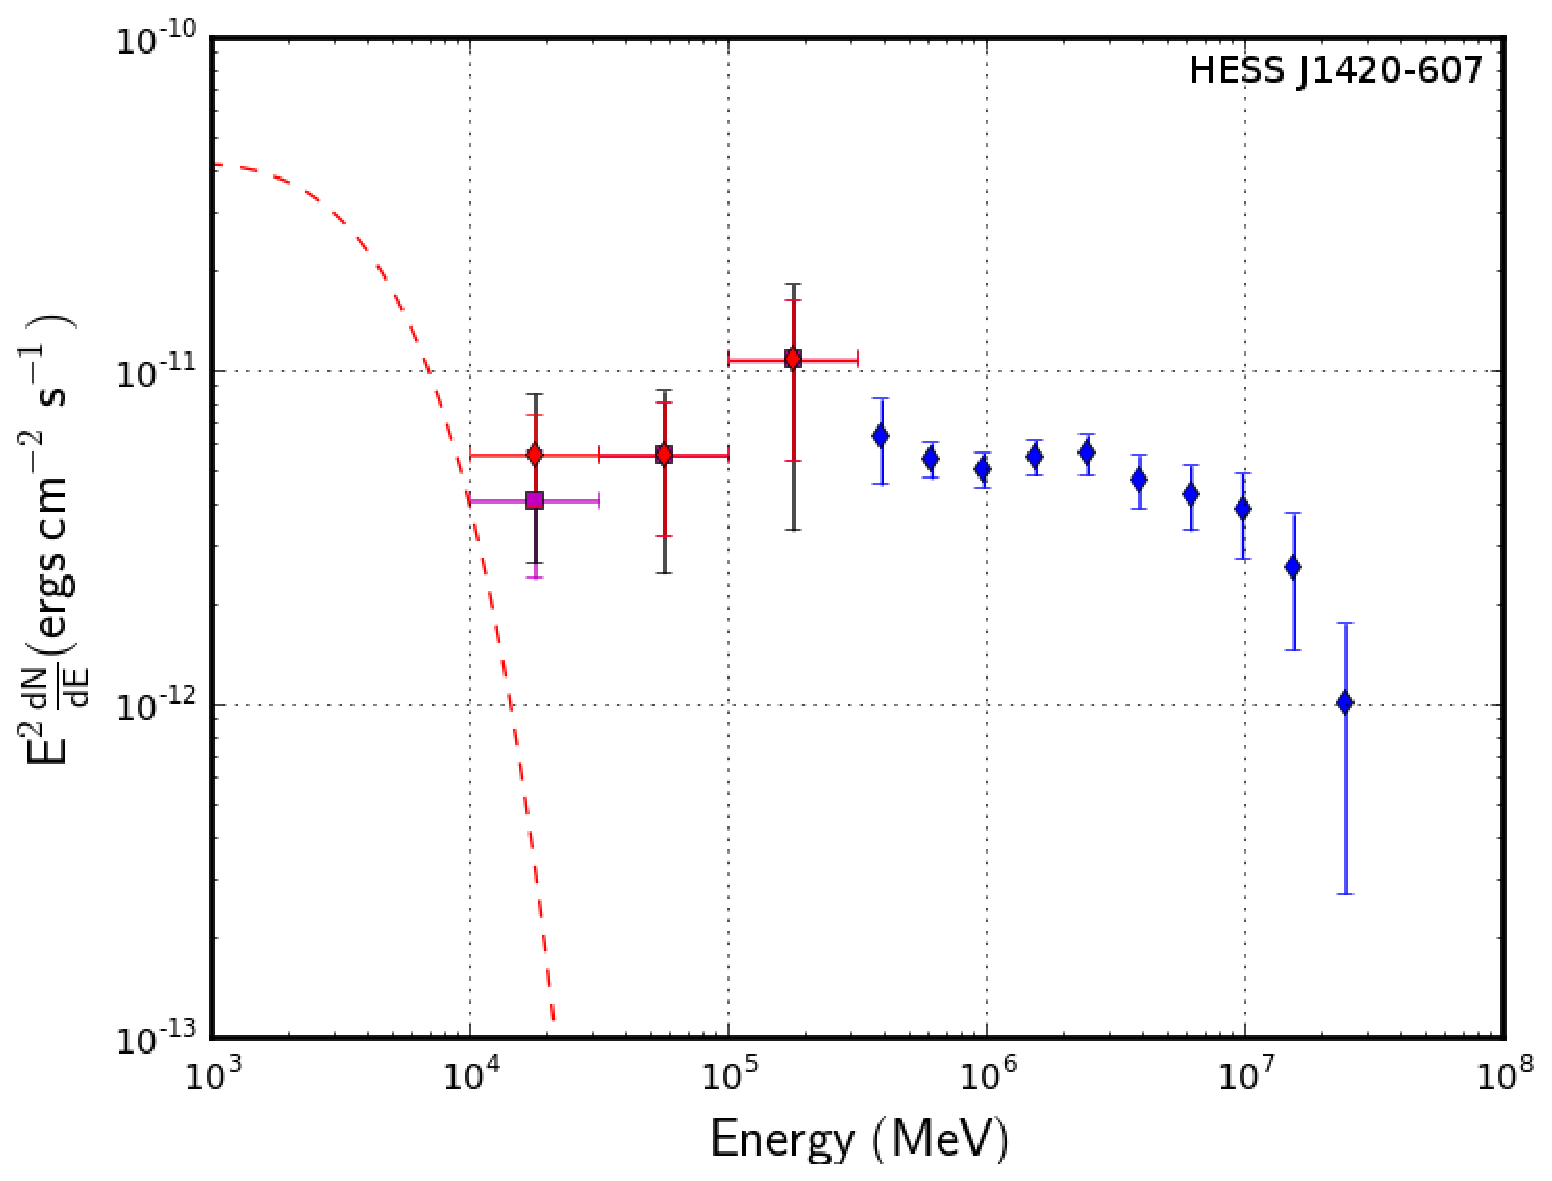
\includegraphics[width=0.60\textwidth]{figures/HESSJ1420.eps}
\label{fig:hessj1420}}
\subfigure{
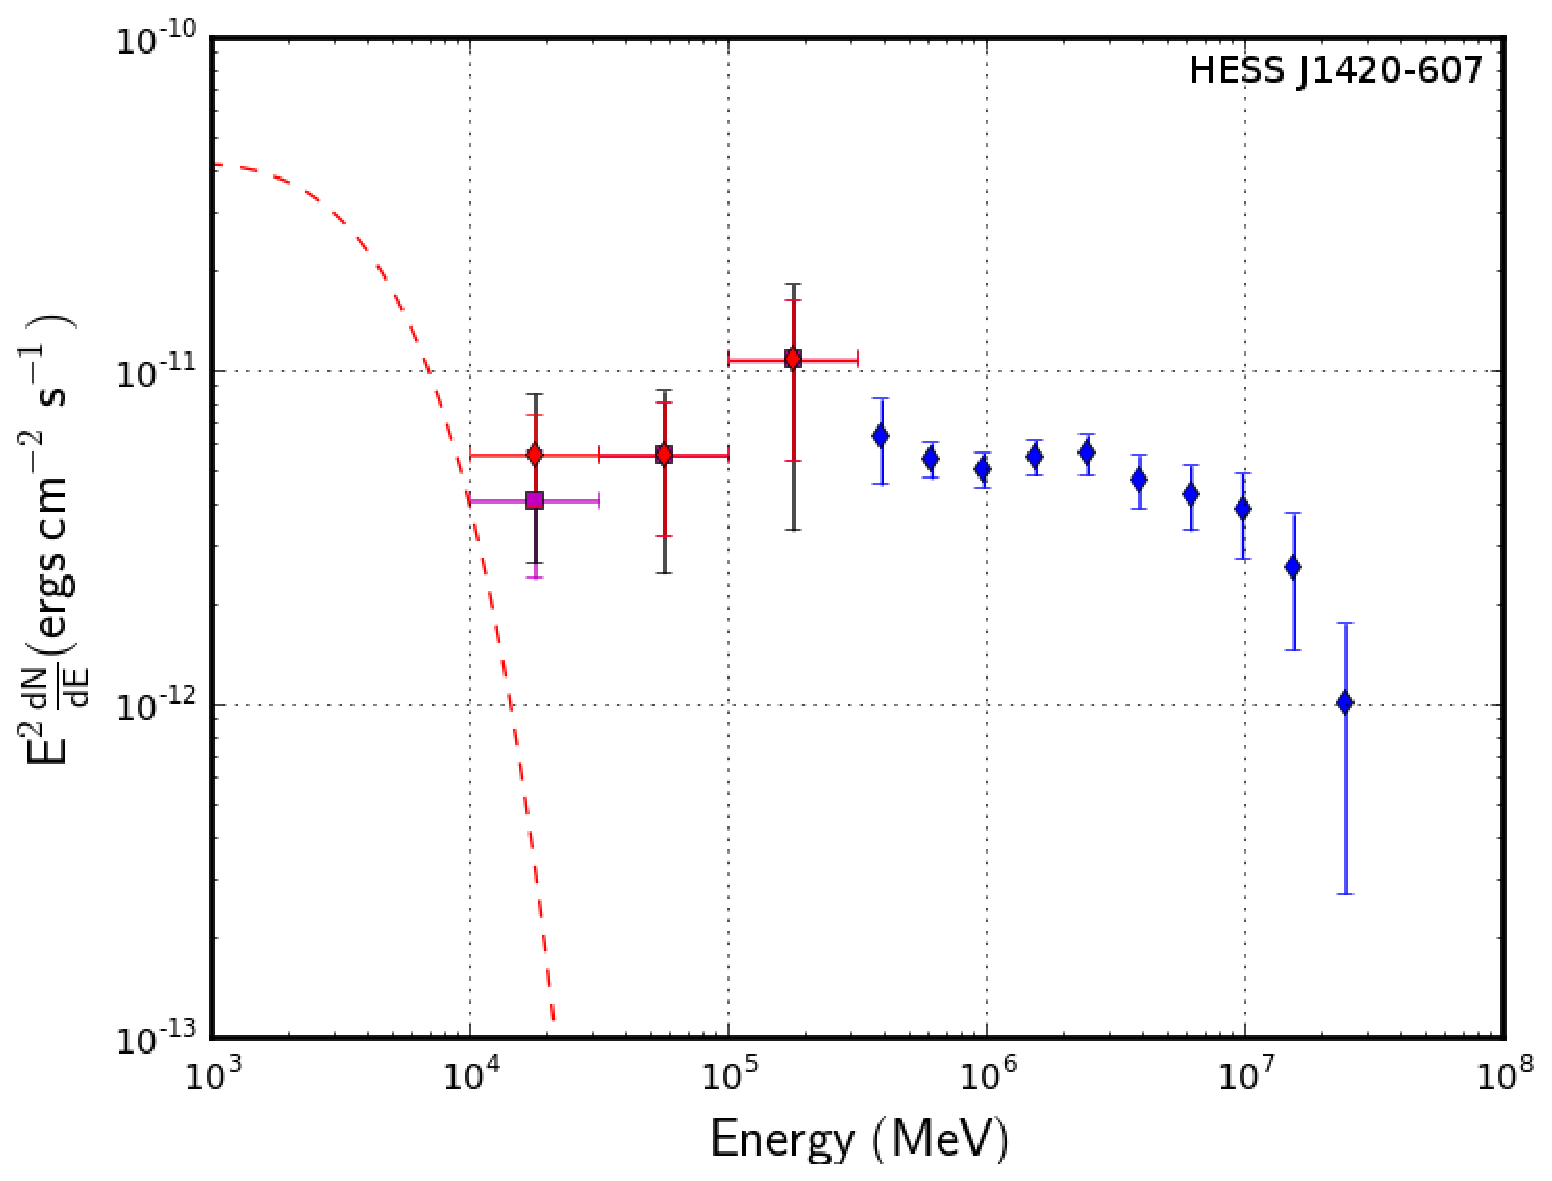
\includegraphics[width=0.60\textwidth]{figures/HESSJ1420.eps}
\label{fig:hessj1420hadro}}
\caption{SED of . Top : Leptonic scenario. Bottom : Hadronic scenario. 
}
\end{figure}

\begin{figure}[h!]
\centering
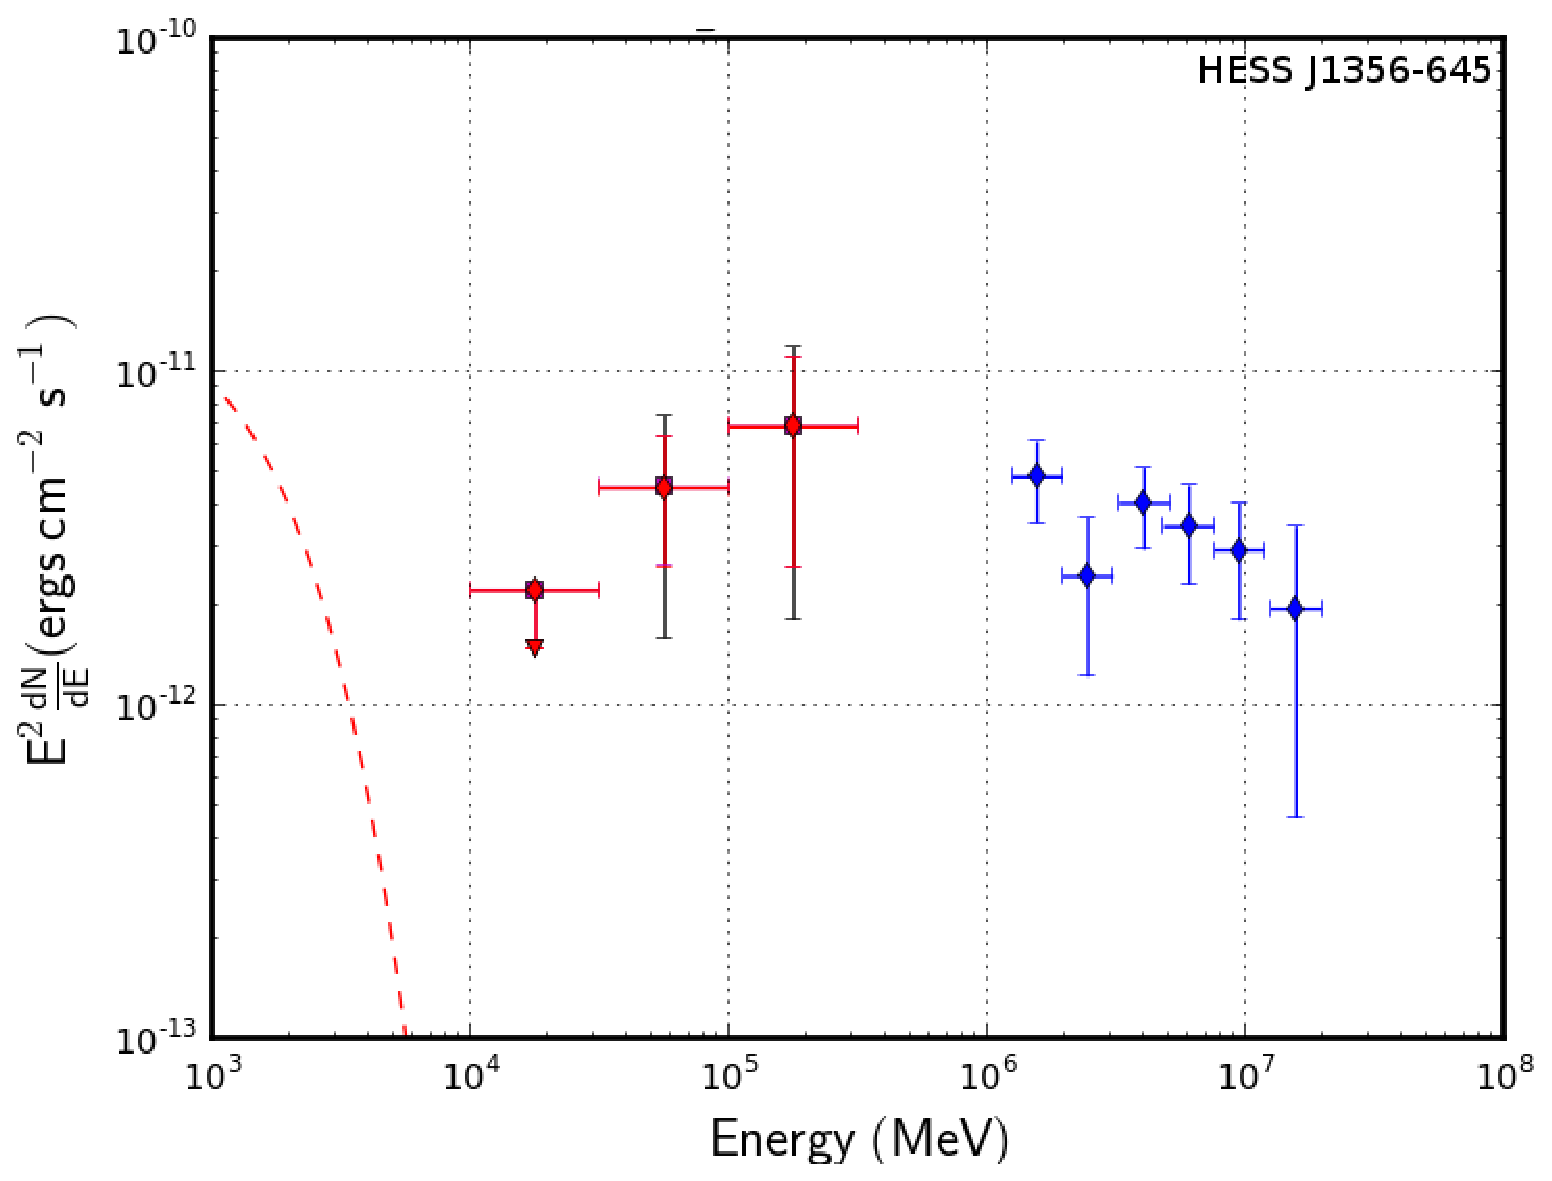
\includegraphics[width=0.60\textwidth]{figures/HESSJ1356.eps}
\caption{SED of
\label{fig:hess1356}}
\end{figure}

\begin{figure}[h!]
\centering
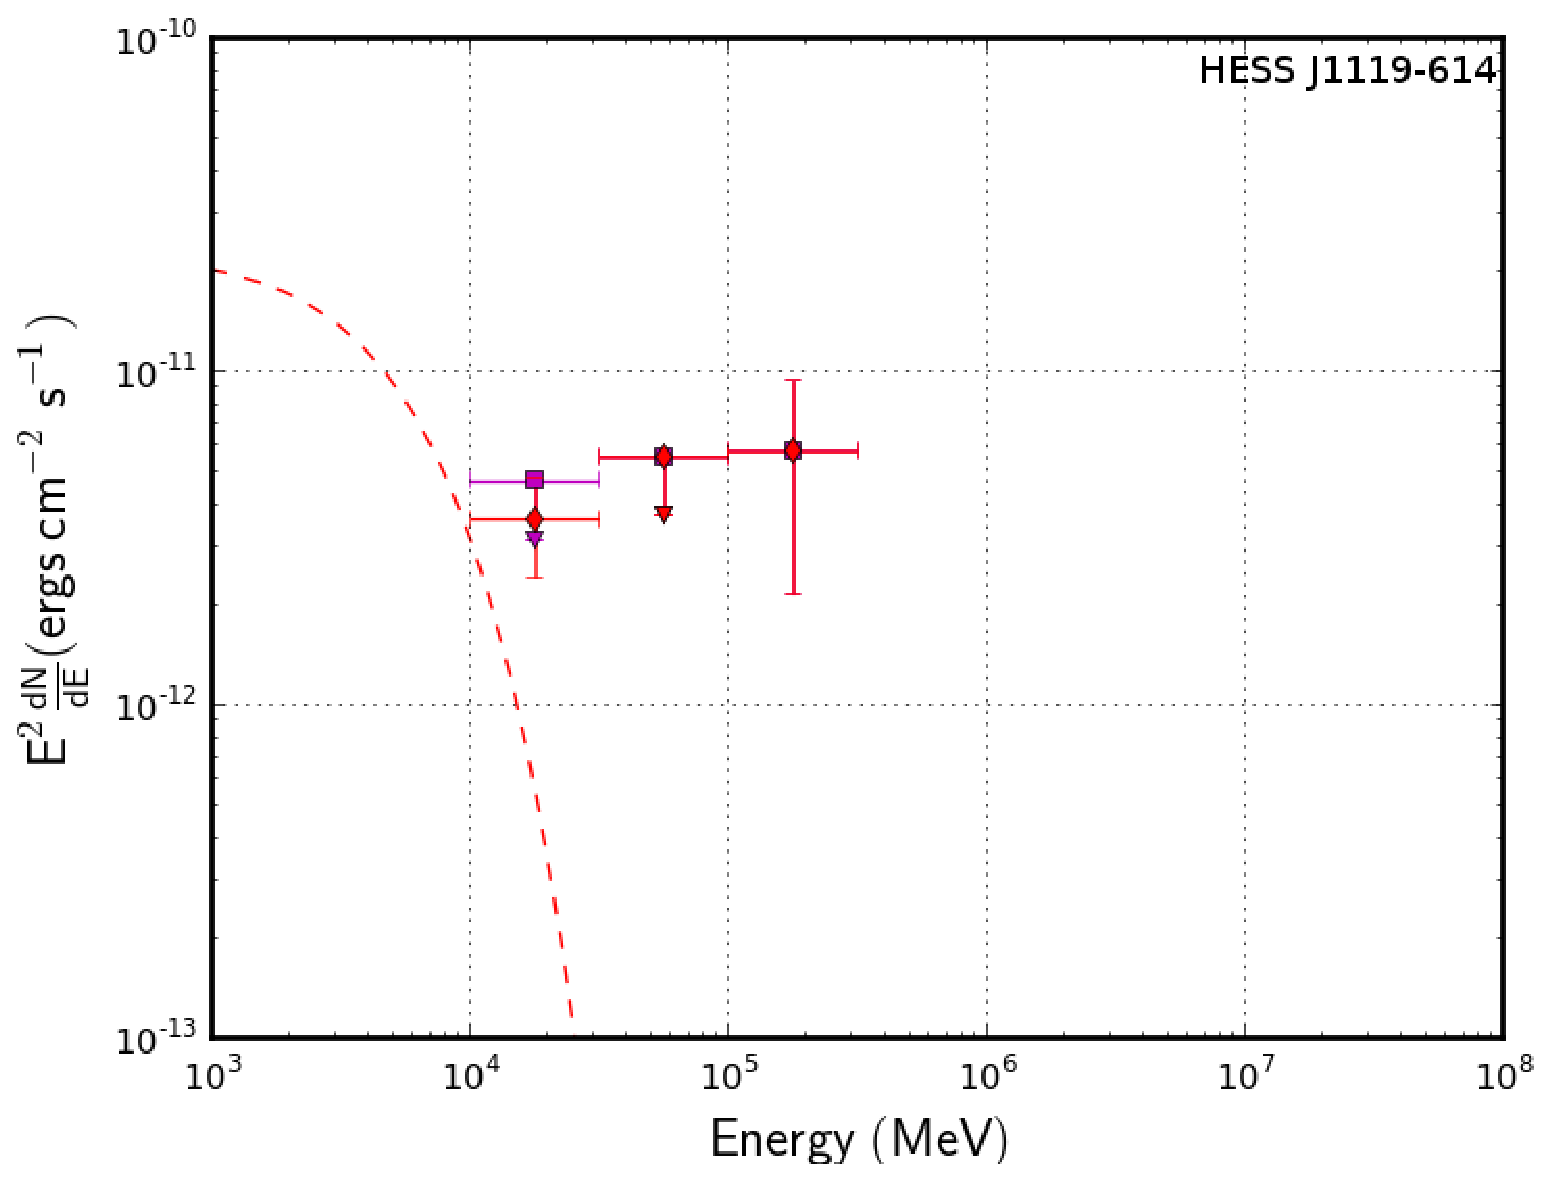
\includegraphics[width=0.60\textwidth]{figures/HESSJ1119.eps}
\caption{SED of 
\label{fig:hessj1119}}
\end{figure}



\begin{figure}[h!]
\centering
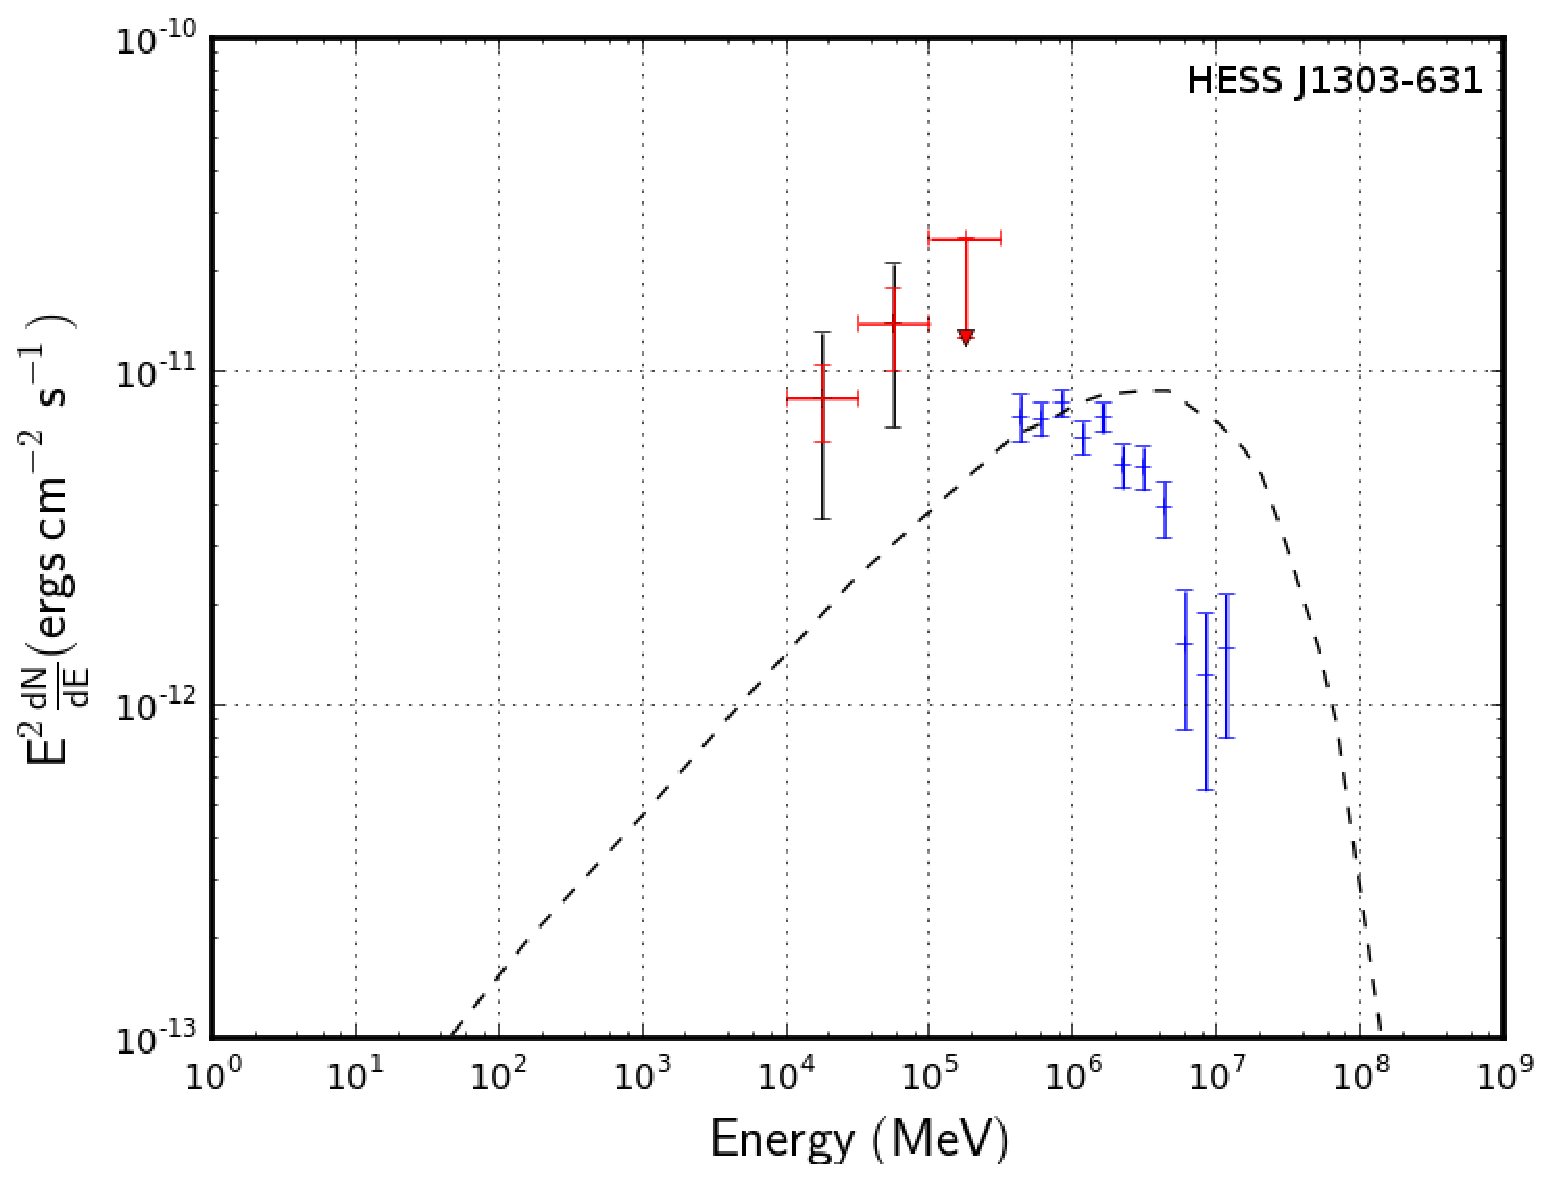
\includegraphics[width=0.60\textwidth]{figures/HESSJ1303631leptdalton.eps}
\caption{SED of 
\label{fig:hessj1303}}
\end{figure}


\begin{figure}[h!]
\centering
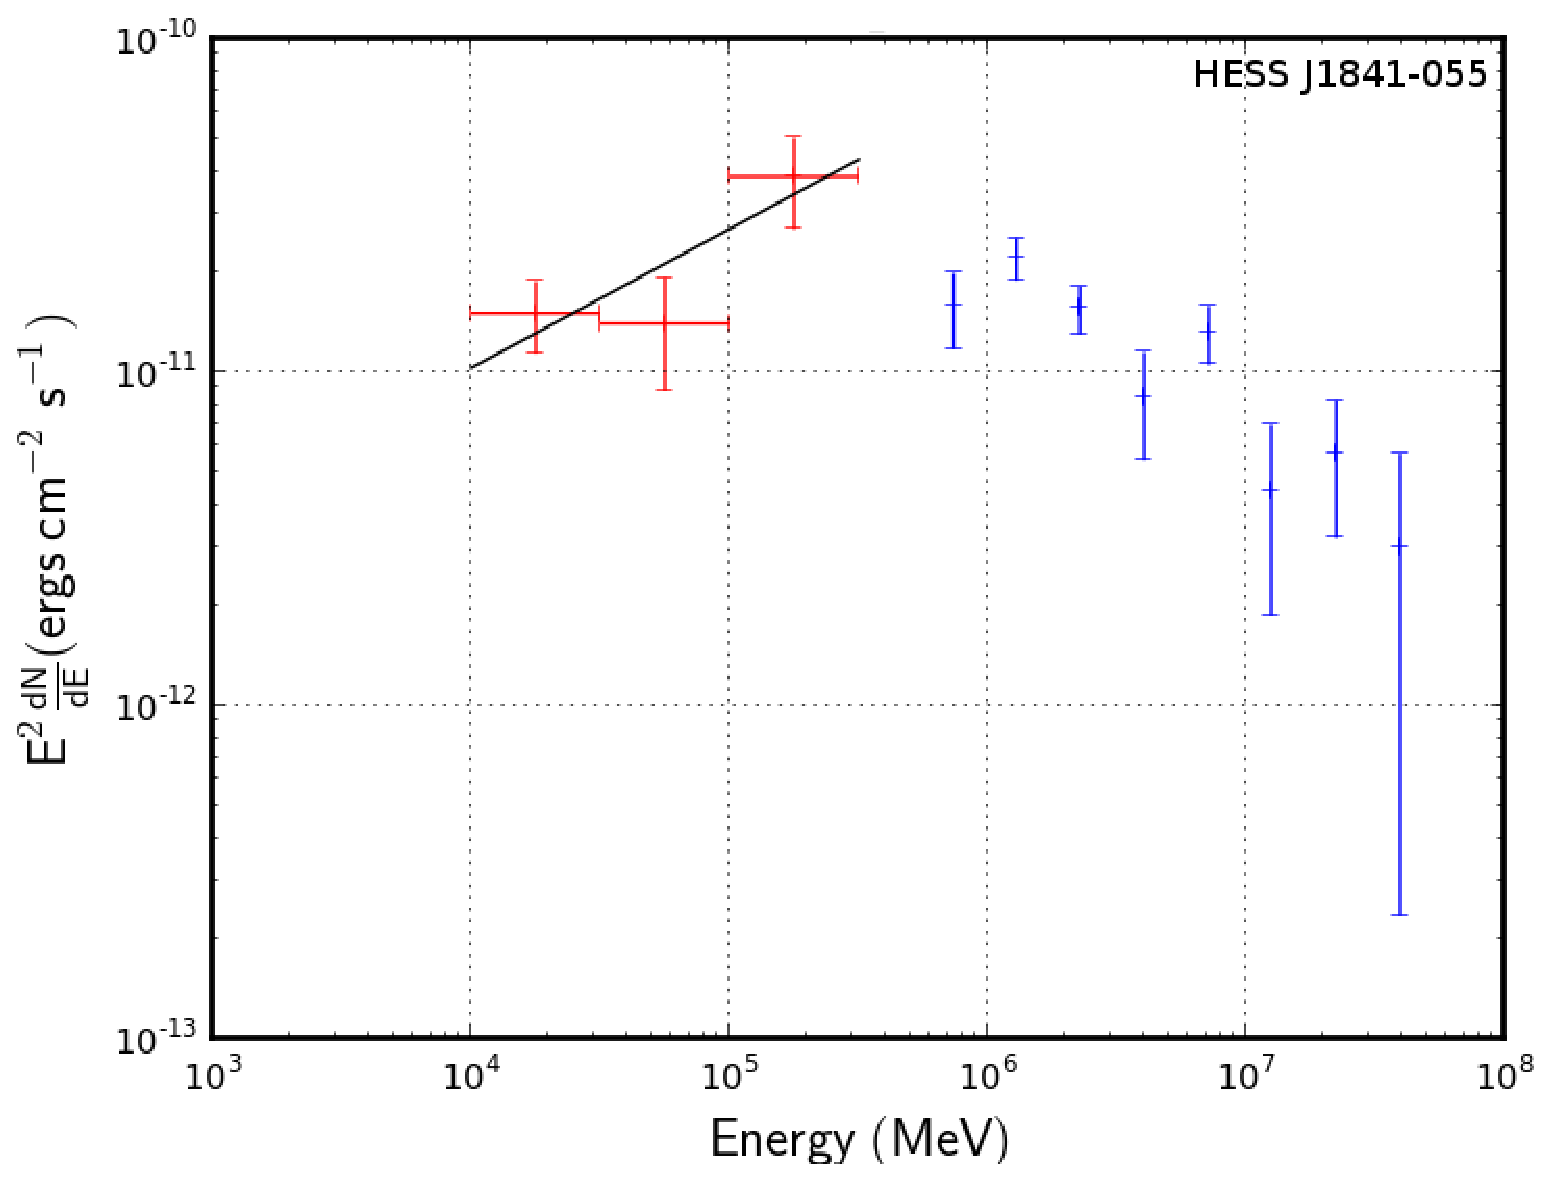
\includegraphics[width=0.60\textwidth]{figures/HESSJ1841055.eps}
\caption{SED of HESS~J1841-055
\label{fig:1841}}
\end{figure}

\begin{figure}[h!]
\centering
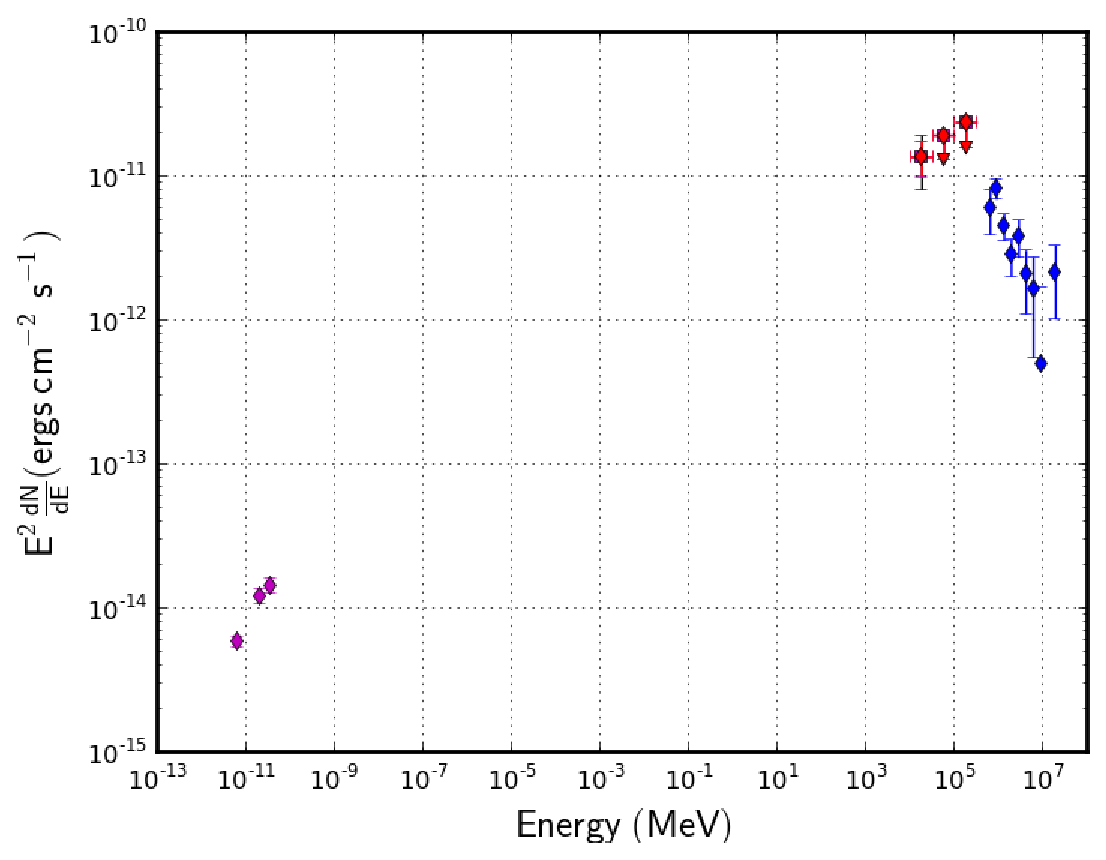
\includegraphics[width=0.60\textwidth]{figures/HESSJ1848.eps}
\caption{SED of HESS~J1848
\label{fig:1848}}
\end{figure}

\begin{figure}[h!]
\centering
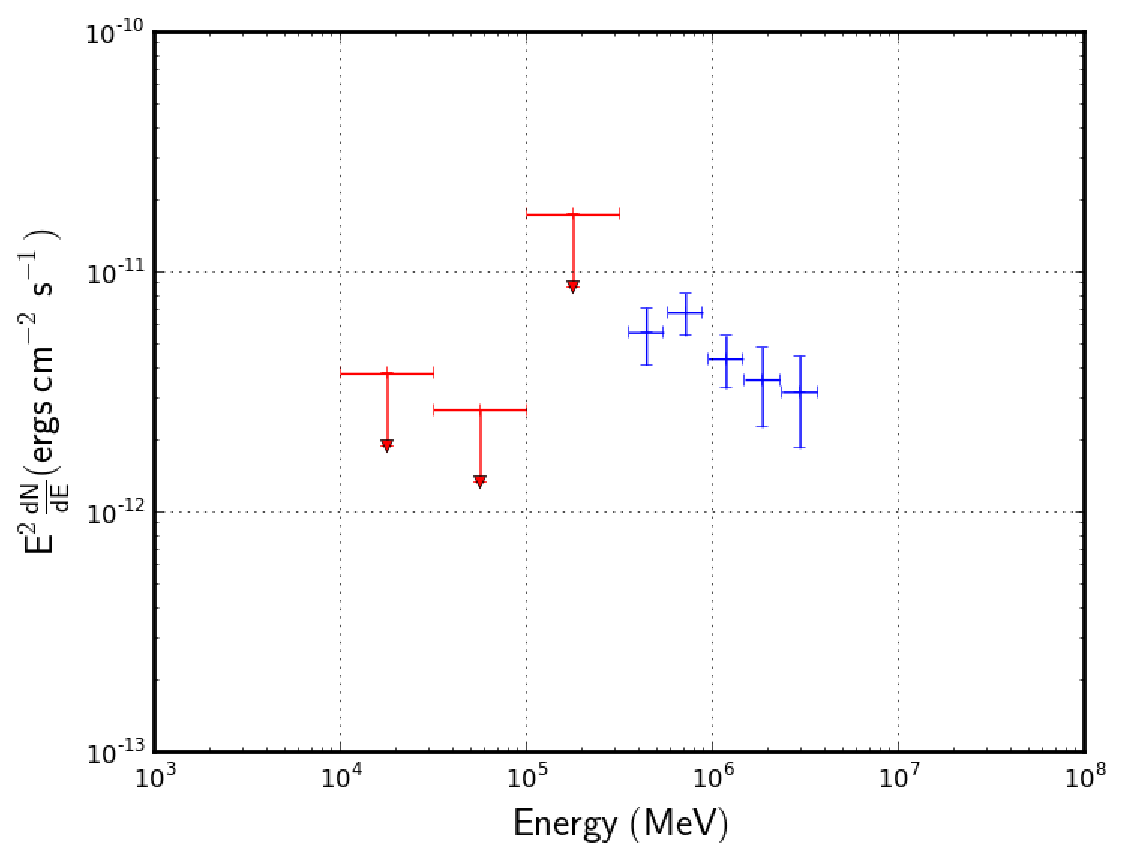
\includegraphics[width=0.60\textwidth]{figures/HESSJ1026.eps}
\caption{SED of HESS~J1026 With SED model
\label{fig:1026}}
\end{figure}

\begin{figure}[h!]
\centering
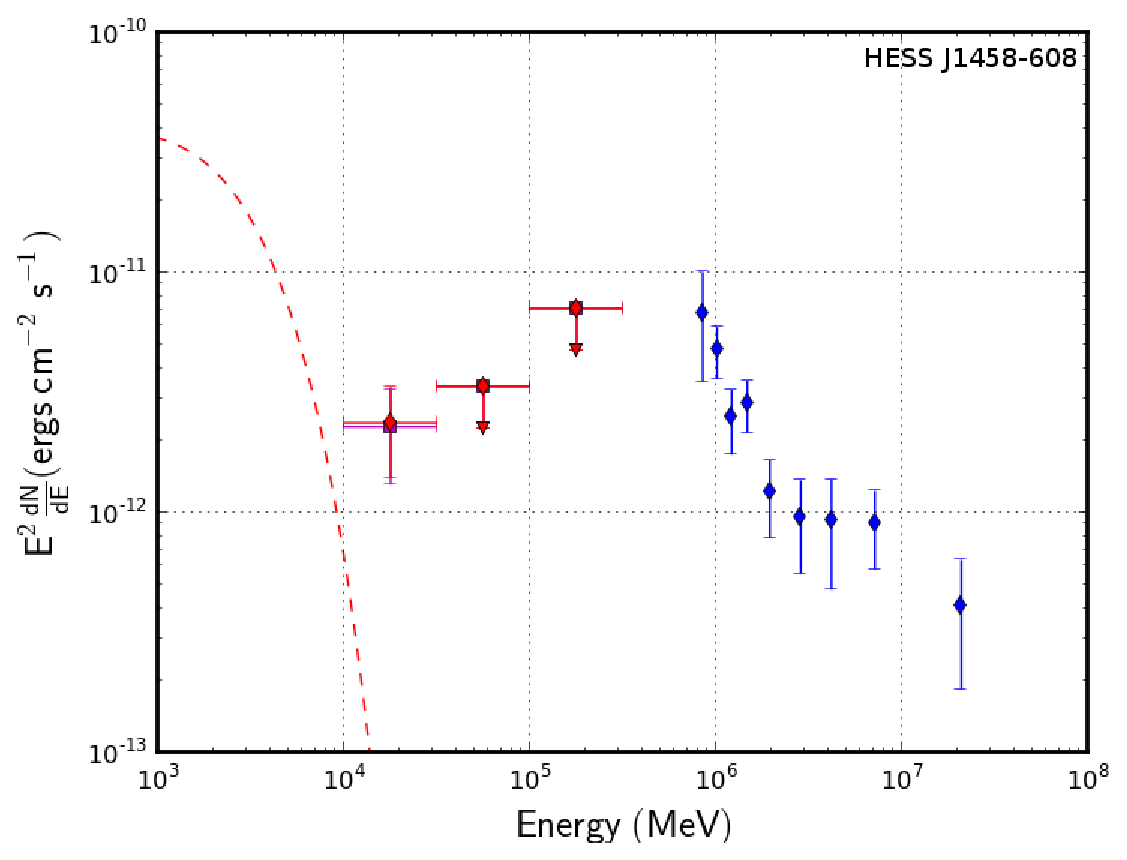
\includegraphics[width=0.60\textwidth]{figures/HESSJ1458.eps}
\caption{SED of HESS~J1458 With SED model
\label{fig:1458}}
\end{figure}

\begin{figure}[h!]
\centering
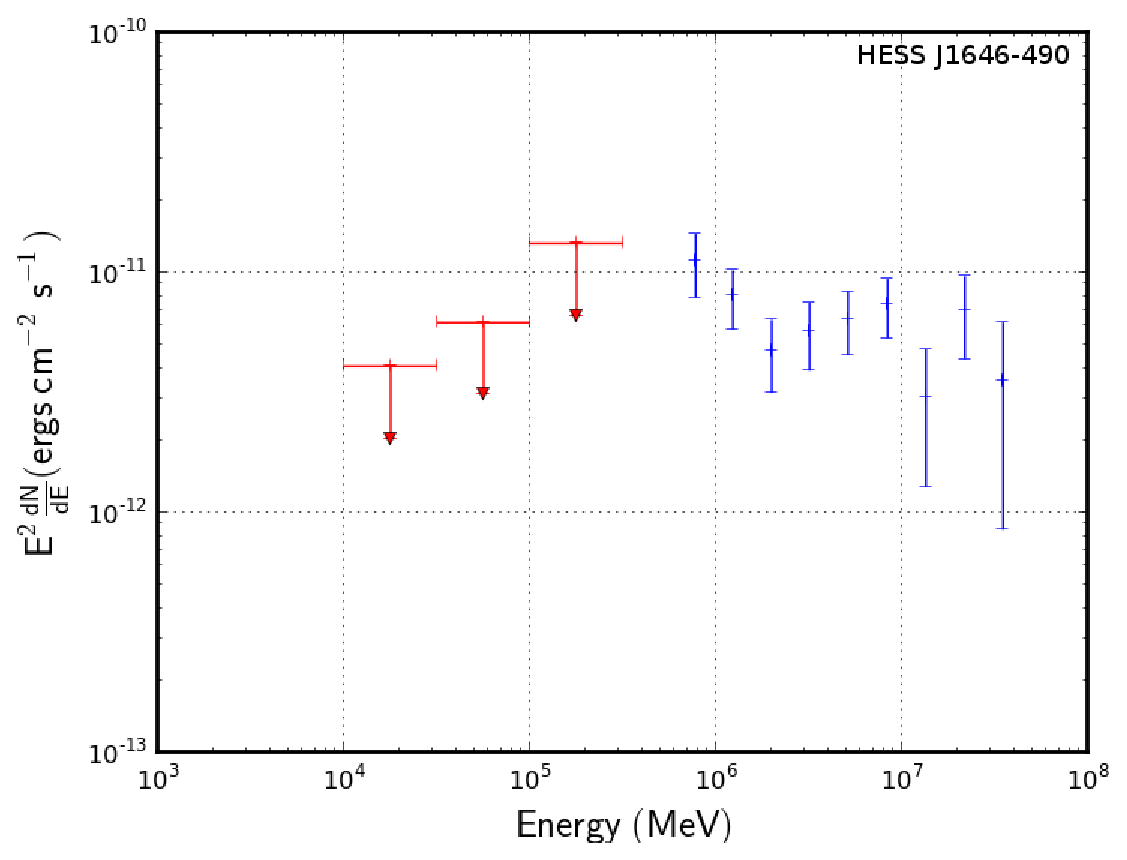
\includegraphics[width=0.60\textwidth]{figures/HESSJ1626.eps}
\caption{SED of HESS~J1626 With SED model
\label{fig:1626}}
\end{figure}

\begin{figure}[h!]
\centering
\subfigure{
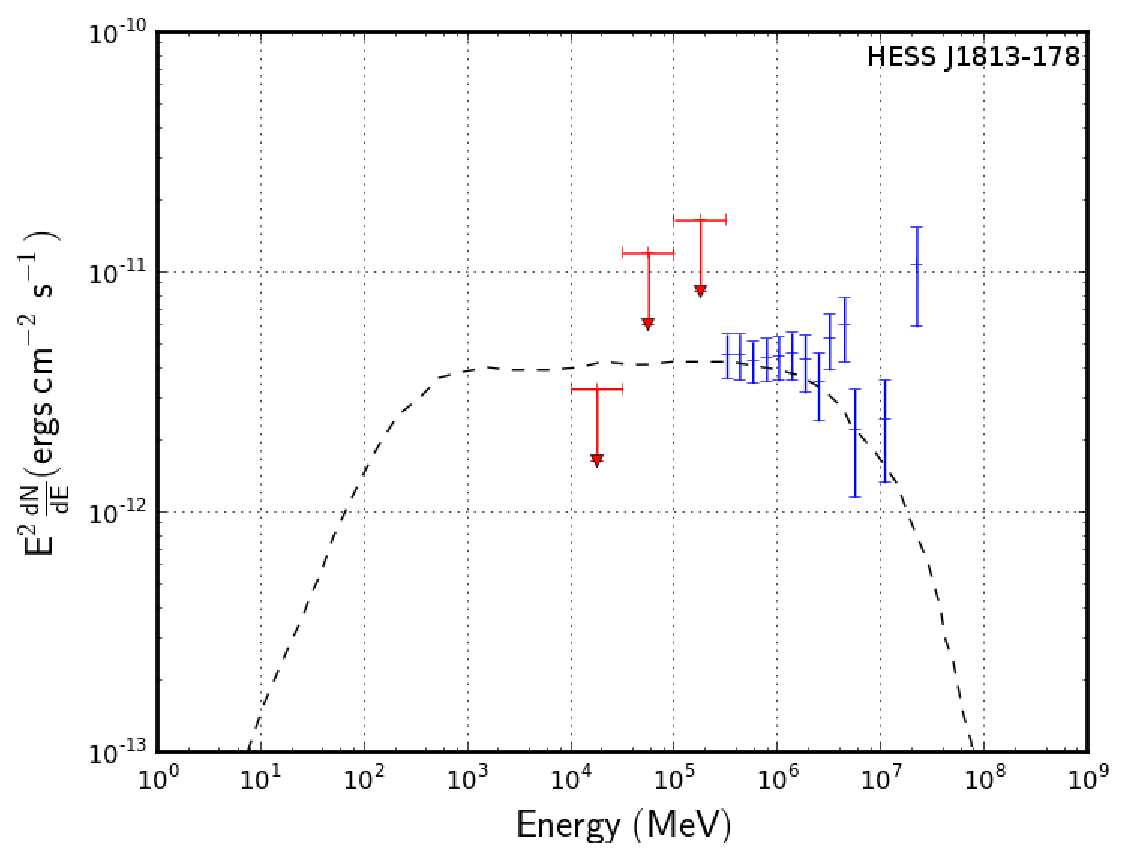
\includegraphics[width=0.60\textwidth]{figures/HESSJ1813178SNRhadron.eps}
\label{fig:hessj1813}}
\subfigure{
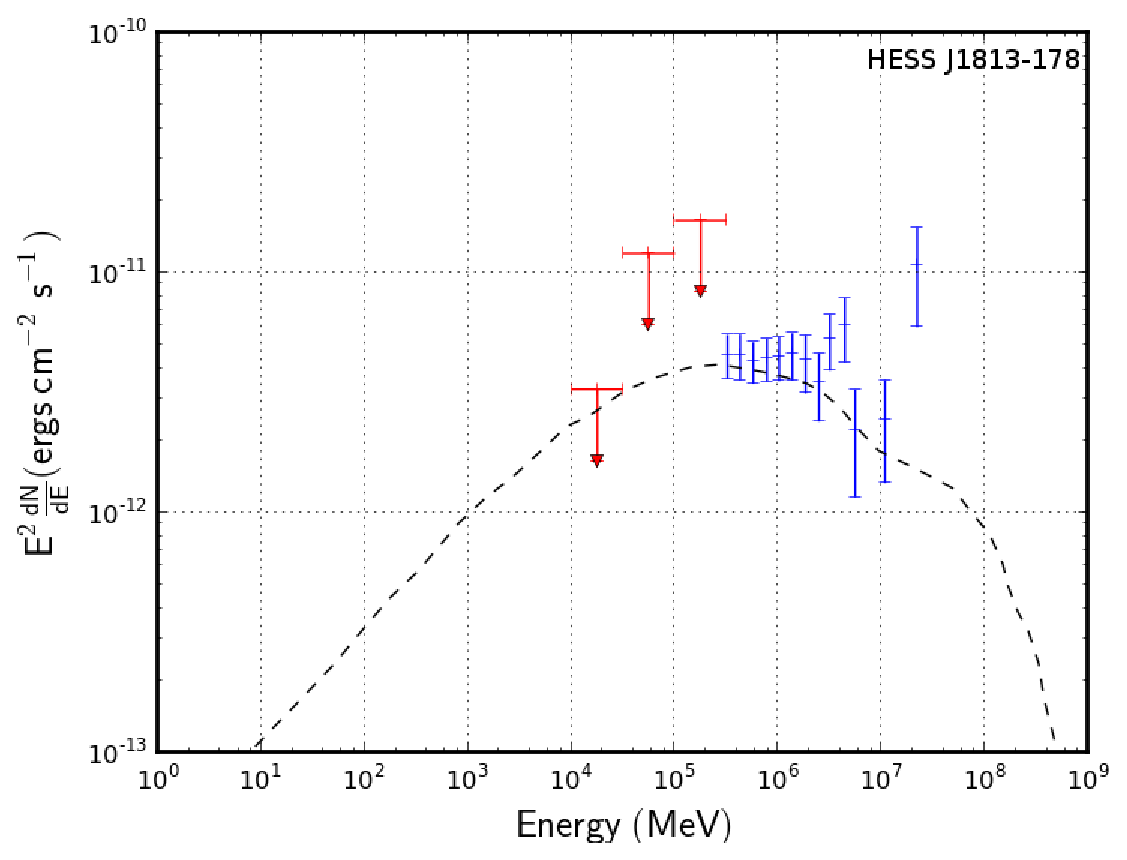
\includegraphics[width=0.60\textwidth]{figures/HESSJ1813178PWNlepton.eps}
\label{fig:hessj1813hadro}}
\caption{SED of . Top : Leptonic scenario. Bottom : Hadronic scenario. 
}

\end{figure}